\chapter{Resultados para dos sigmoides}\label{anx:2}
\subsection*{Variando el parámetro $r_{ig,max}$}

\begin{figure}[htbp]
  \centering
  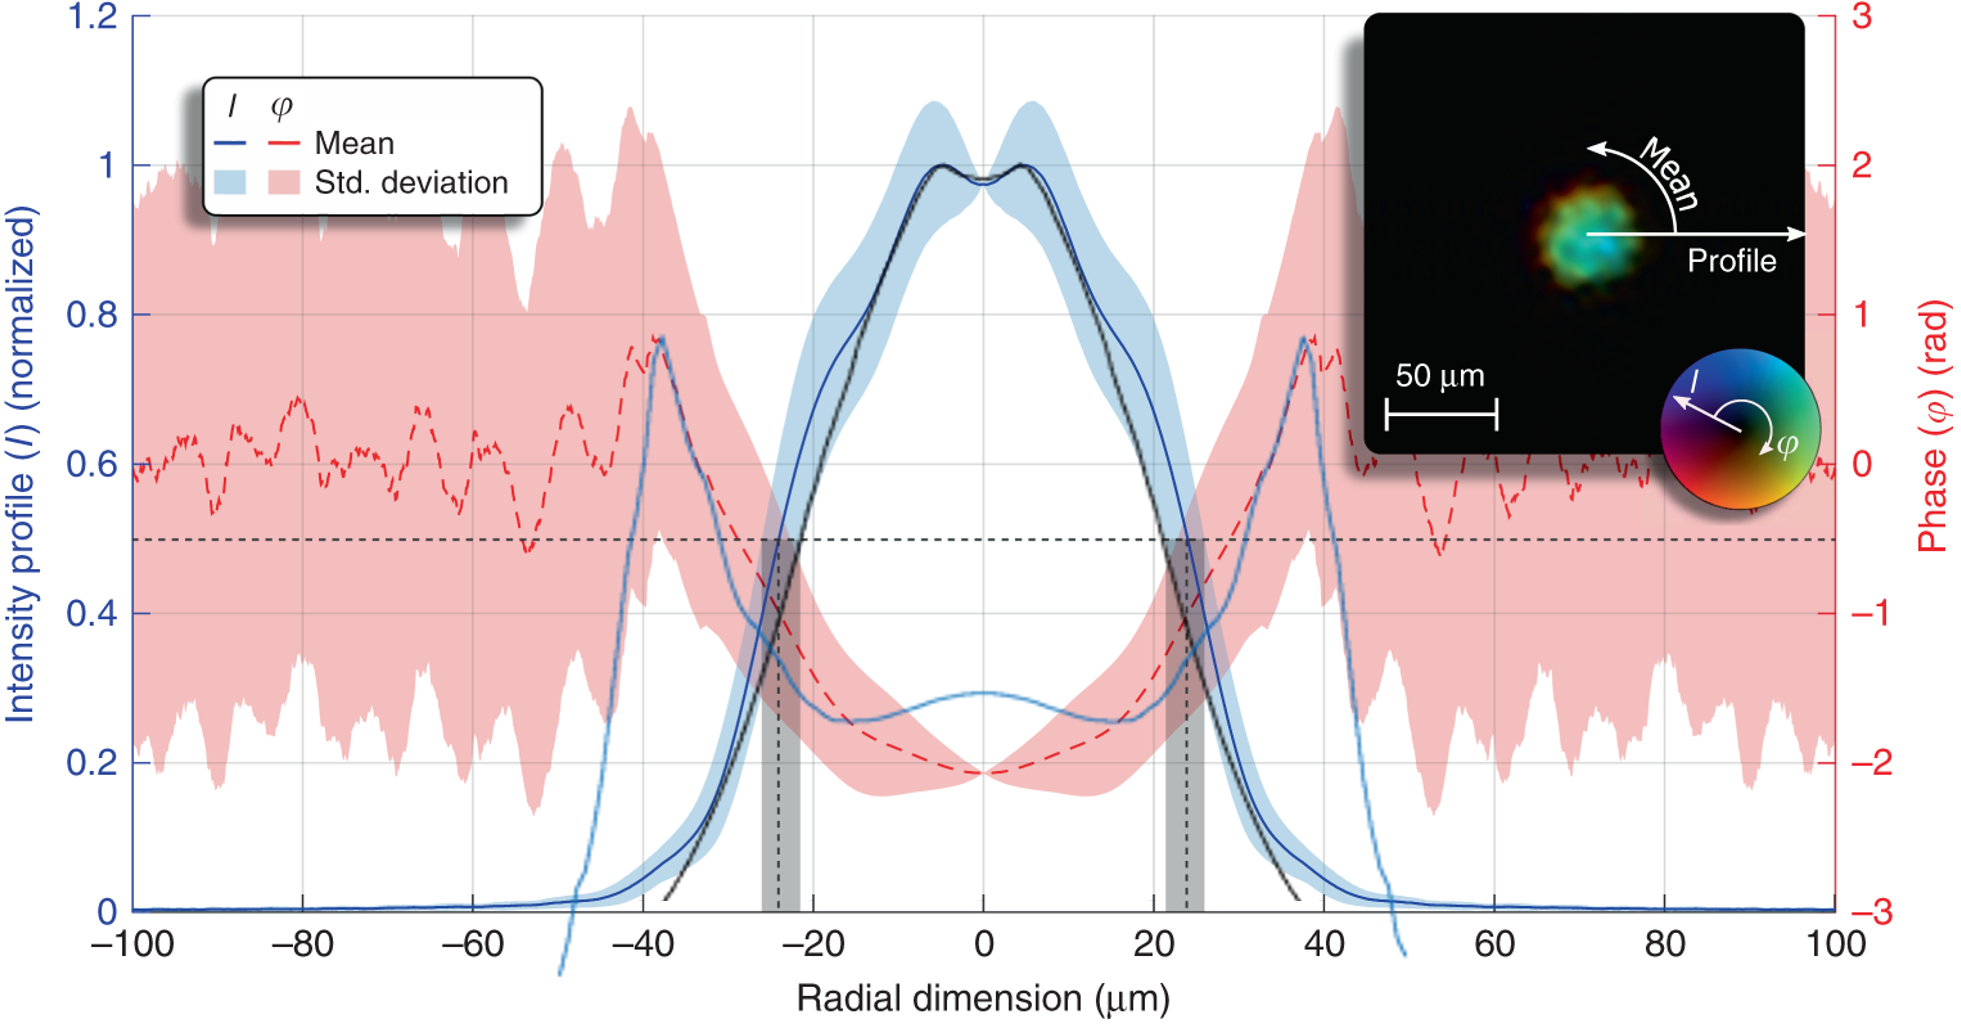
\includegraphics[width=0.75\textwidth]{Figuras/anx_cmp_51.png}
  \caption*{Comparación entre los perfiles radiales de intensidad--fase con $r_{ig,min}=r_{ig,max}=\qty{15}{µm}$, manteniendo los valores de los parámetros $k_{ig}=\qty{5000}{m^{-1}}$ y $z_{0ig}=\qty{4}{mm}$; y el experimento.}
\end{figure}

\begin{figure}[htbp]
  \centering
  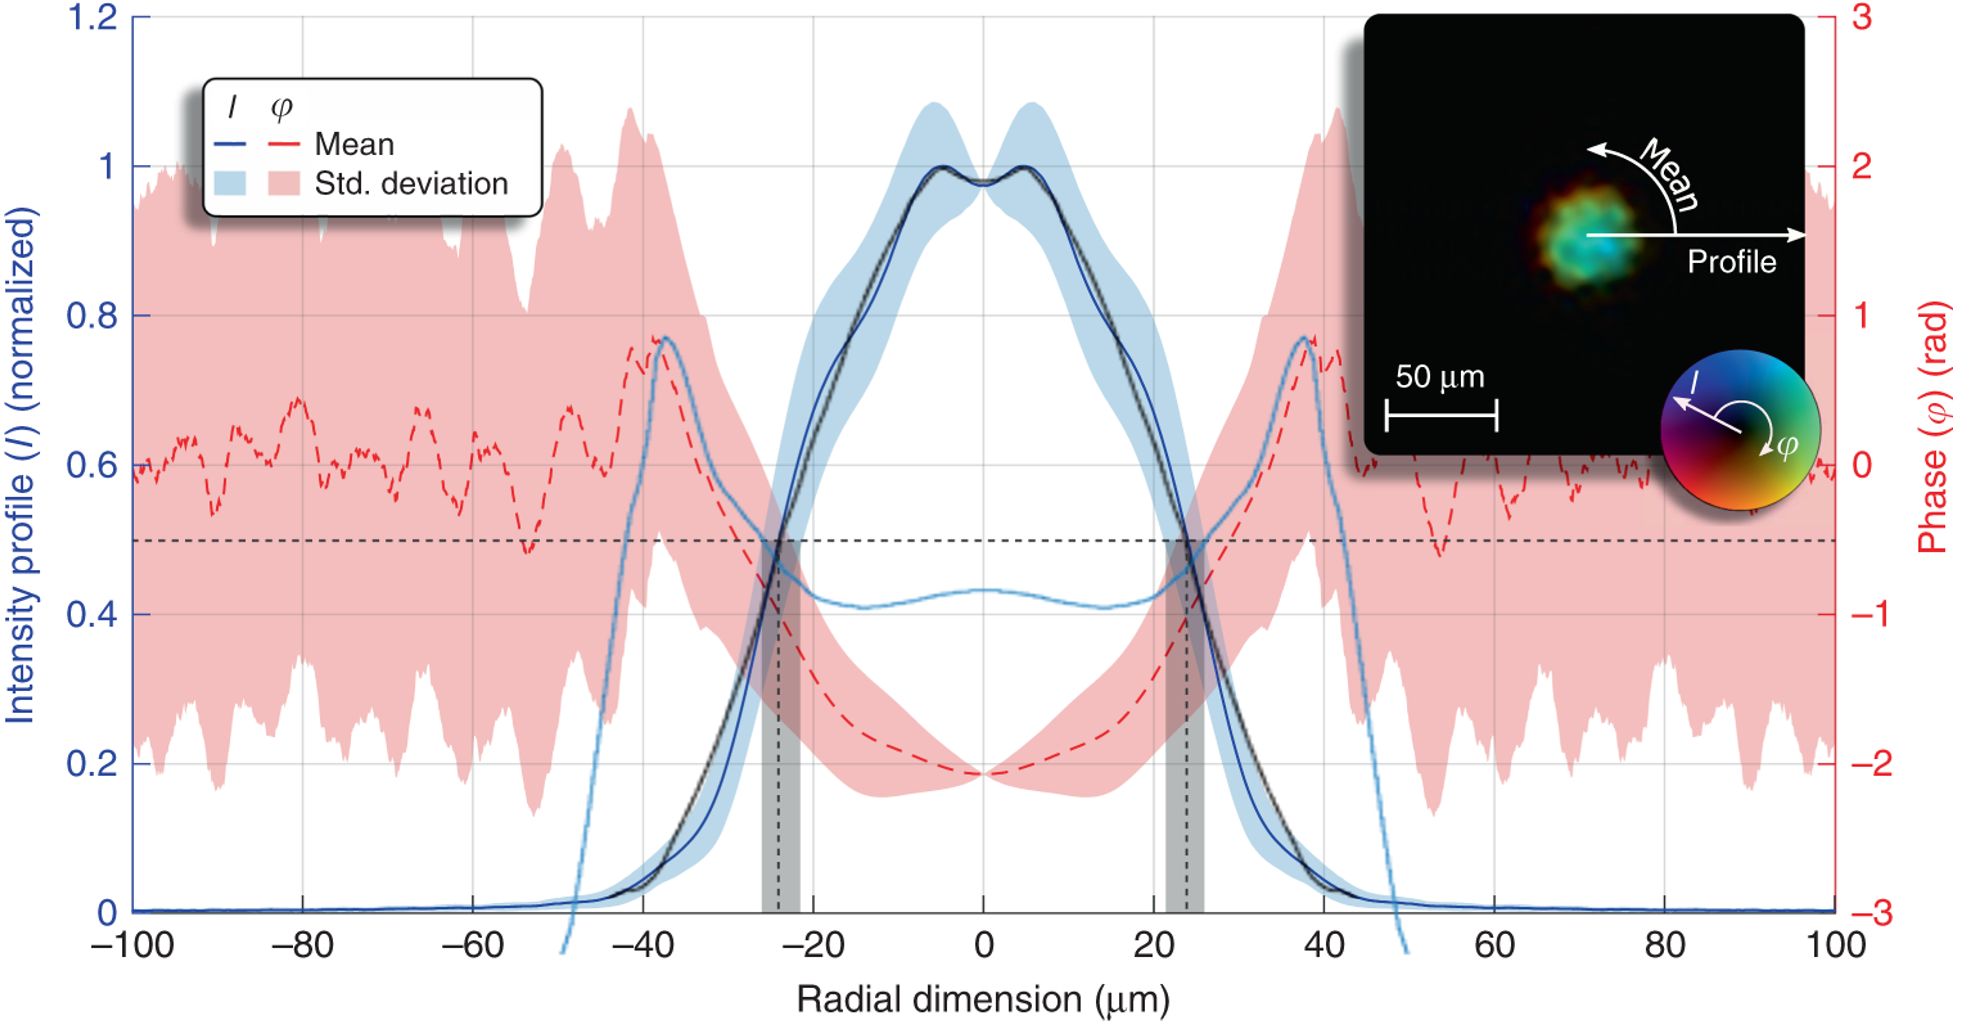
\includegraphics[width=0.75\textwidth]{Figuras/anx_cmp_52.png}
  \caption*{Comparación entre los perfiles radiales de intensidad--fase con $r_{ig,min}=\qty{15}{µm}$ y $r_{ig,max}=\qty{17}{µm}$, manteniendo los valores de los parámetros $k_{ig}=\qty{5000}{m^{-1}}$ y $z_{0ig}=\qty{4}{mm}$; y el experimento.}
\end{figure}

\begin{figure}[htbp]
  \centering
  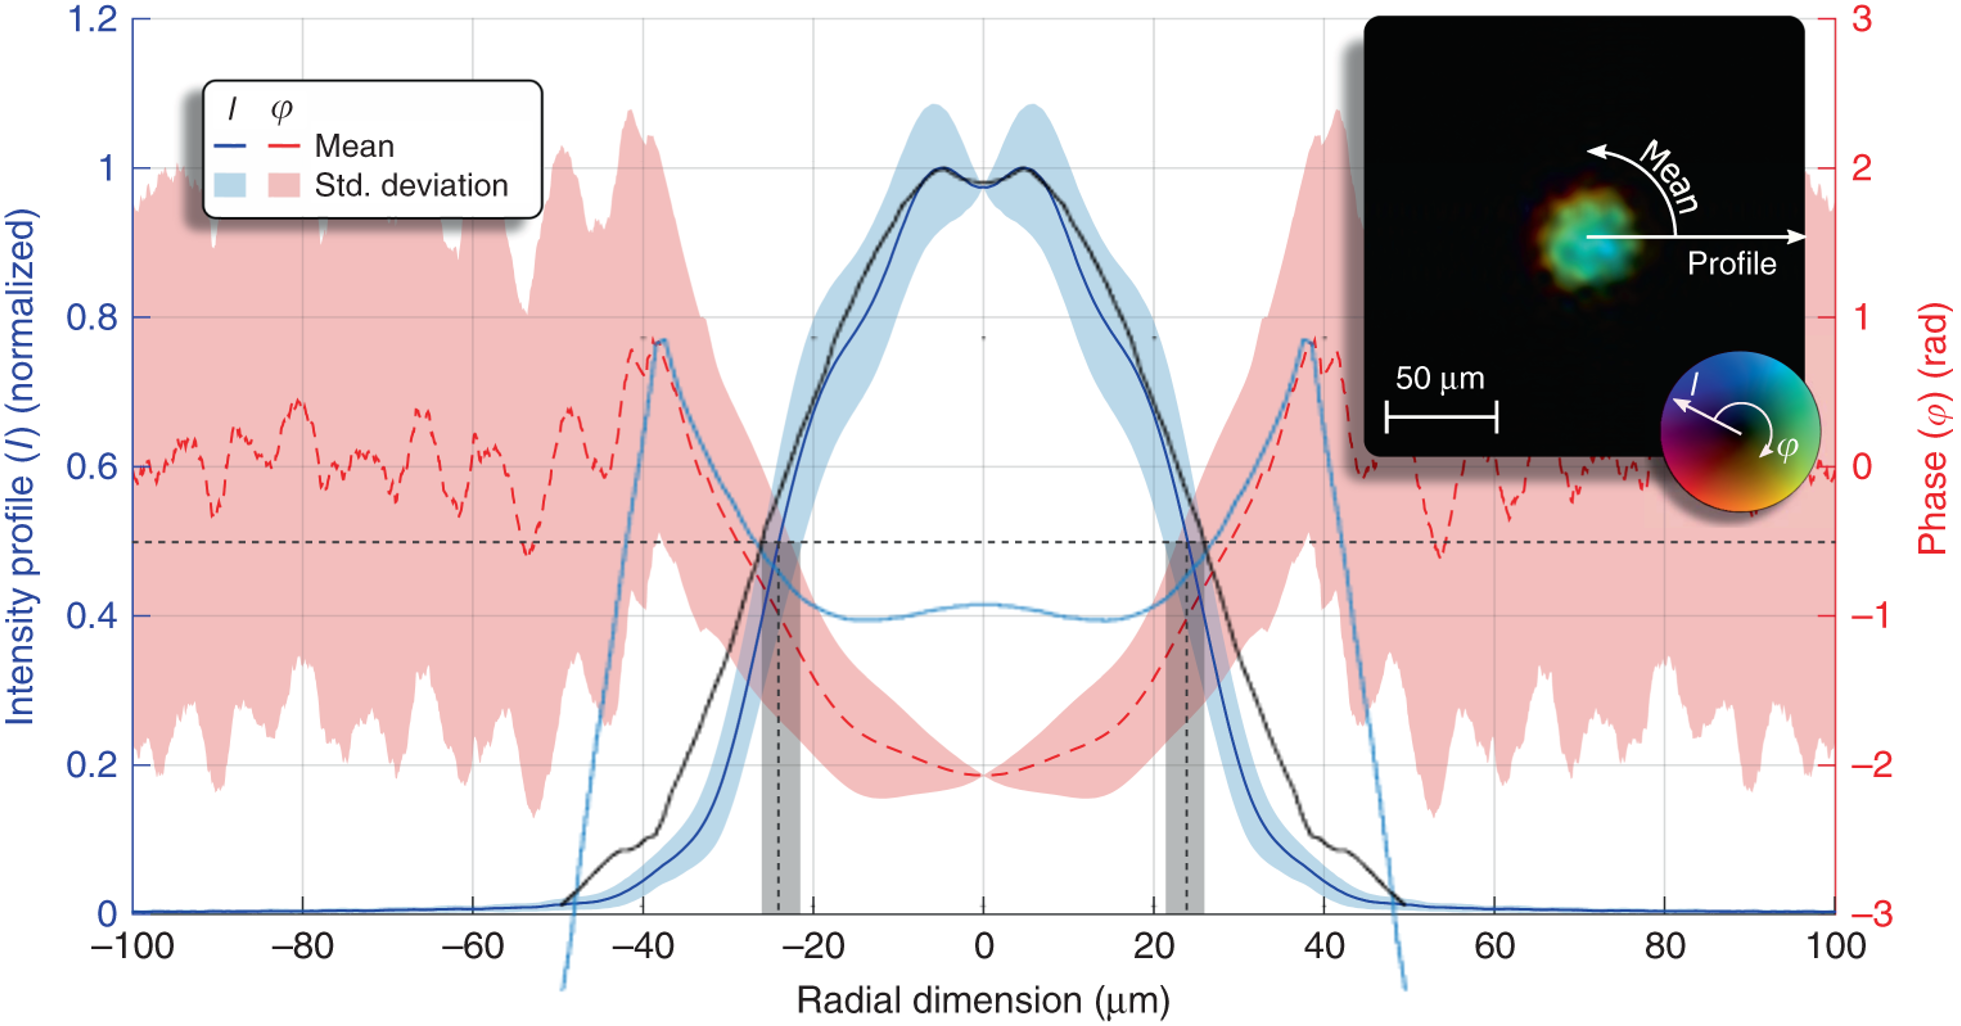
\includegraphics[width=0.74\textwidth]{Figuras/anx_cmp_53.png}
  \caption*{Comparación entre los perfiles radiales de intensidad--fase con $r_{ig,min}=\qty{15}{µm}$ y $r_{ig,max}=\qty{19}{µm}$, manteniendo los valores de los parámetros $k_{ig}=\qty{5000}{m^{-1}}$ y $z_{0ig}=\qty{4}{mm}$; y el experimento.}
\end{figure}

\begin{figure}[htbp]
  \centering
  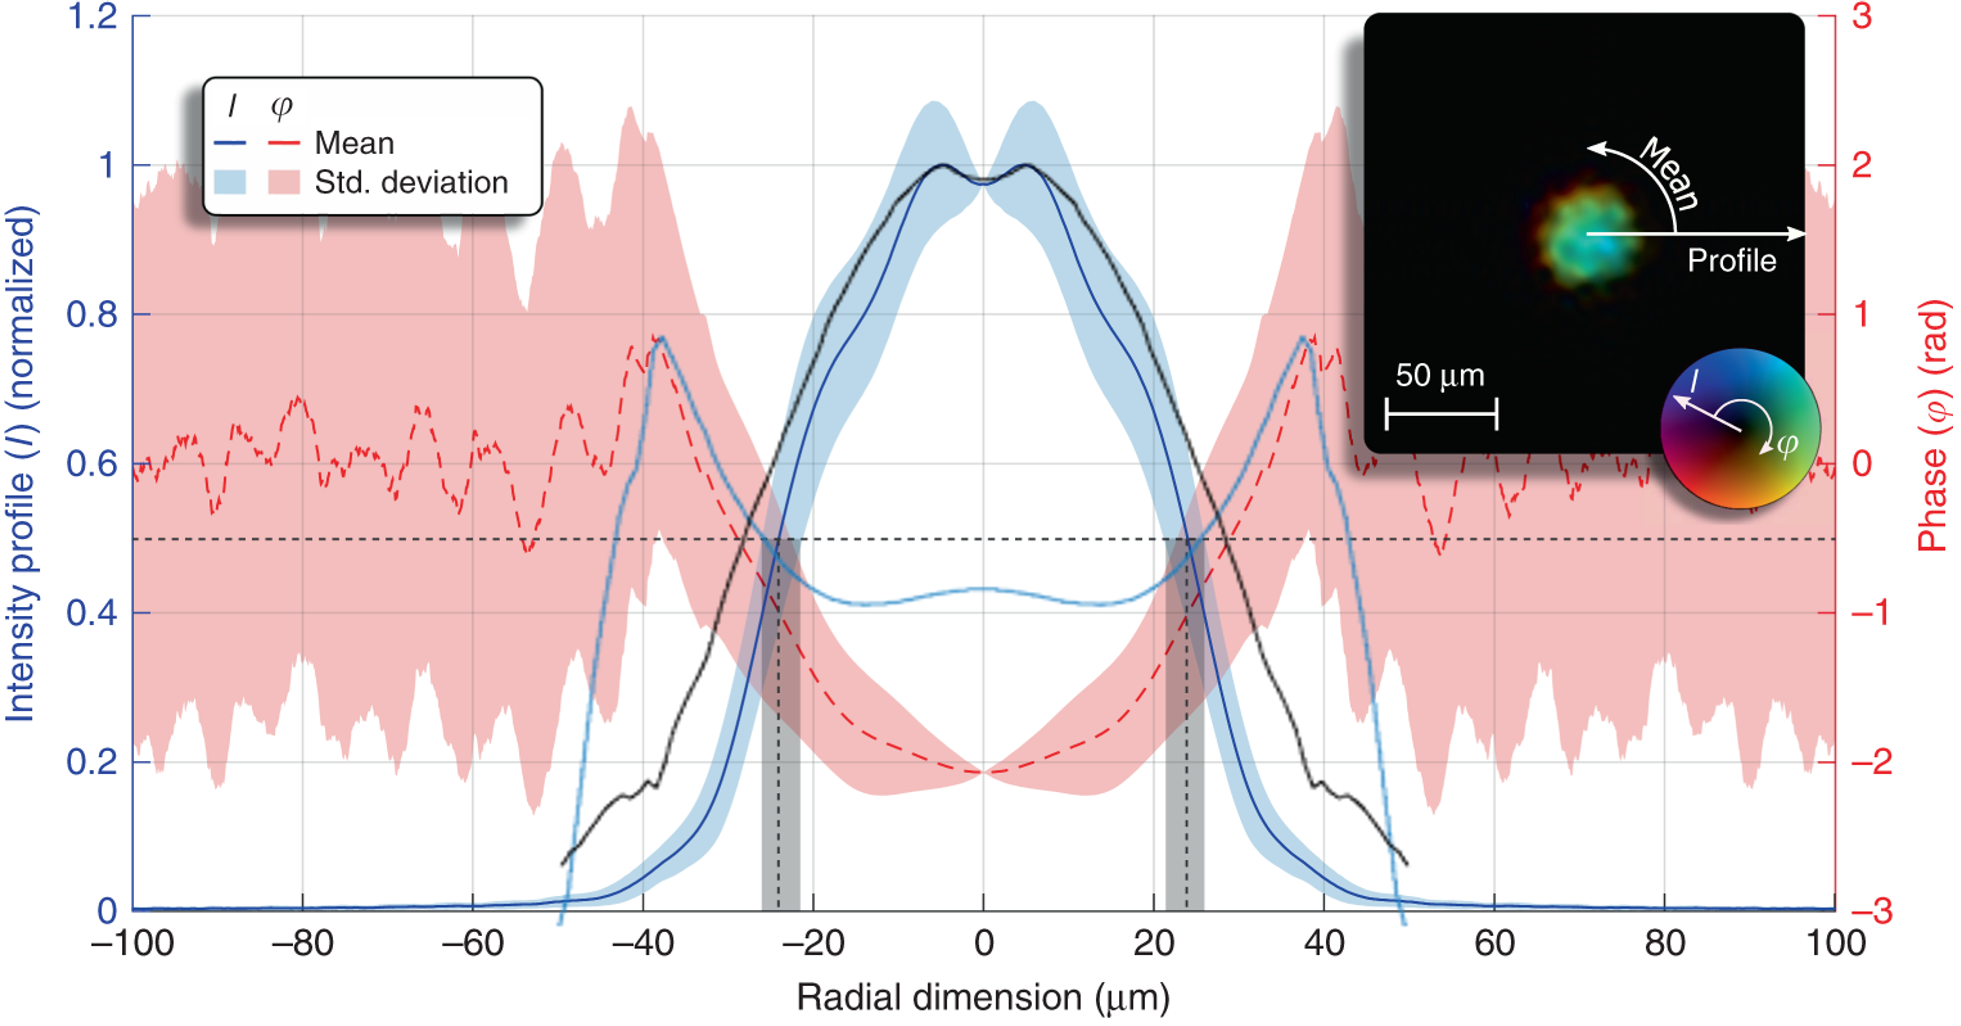
\includegraphics[width=0.74\textwidth]{Figuras/anx_cmp_54.png}
  \caption*{Comparación entre los perfiles radiales de intensidad--fase con $r_{ig,min}=\qty{15}{µm}$ y $r_{ig,max}=\qty{21}{µm}$, manteniendo los valores de los parámetros $k_{ig}=\qty{5000}{m^{-1}}$ y $z_{0ig}=\qty{4}{mm}$; y el experimento.}
\end{figure}

\begin{figure}[htbp]
  \centering
  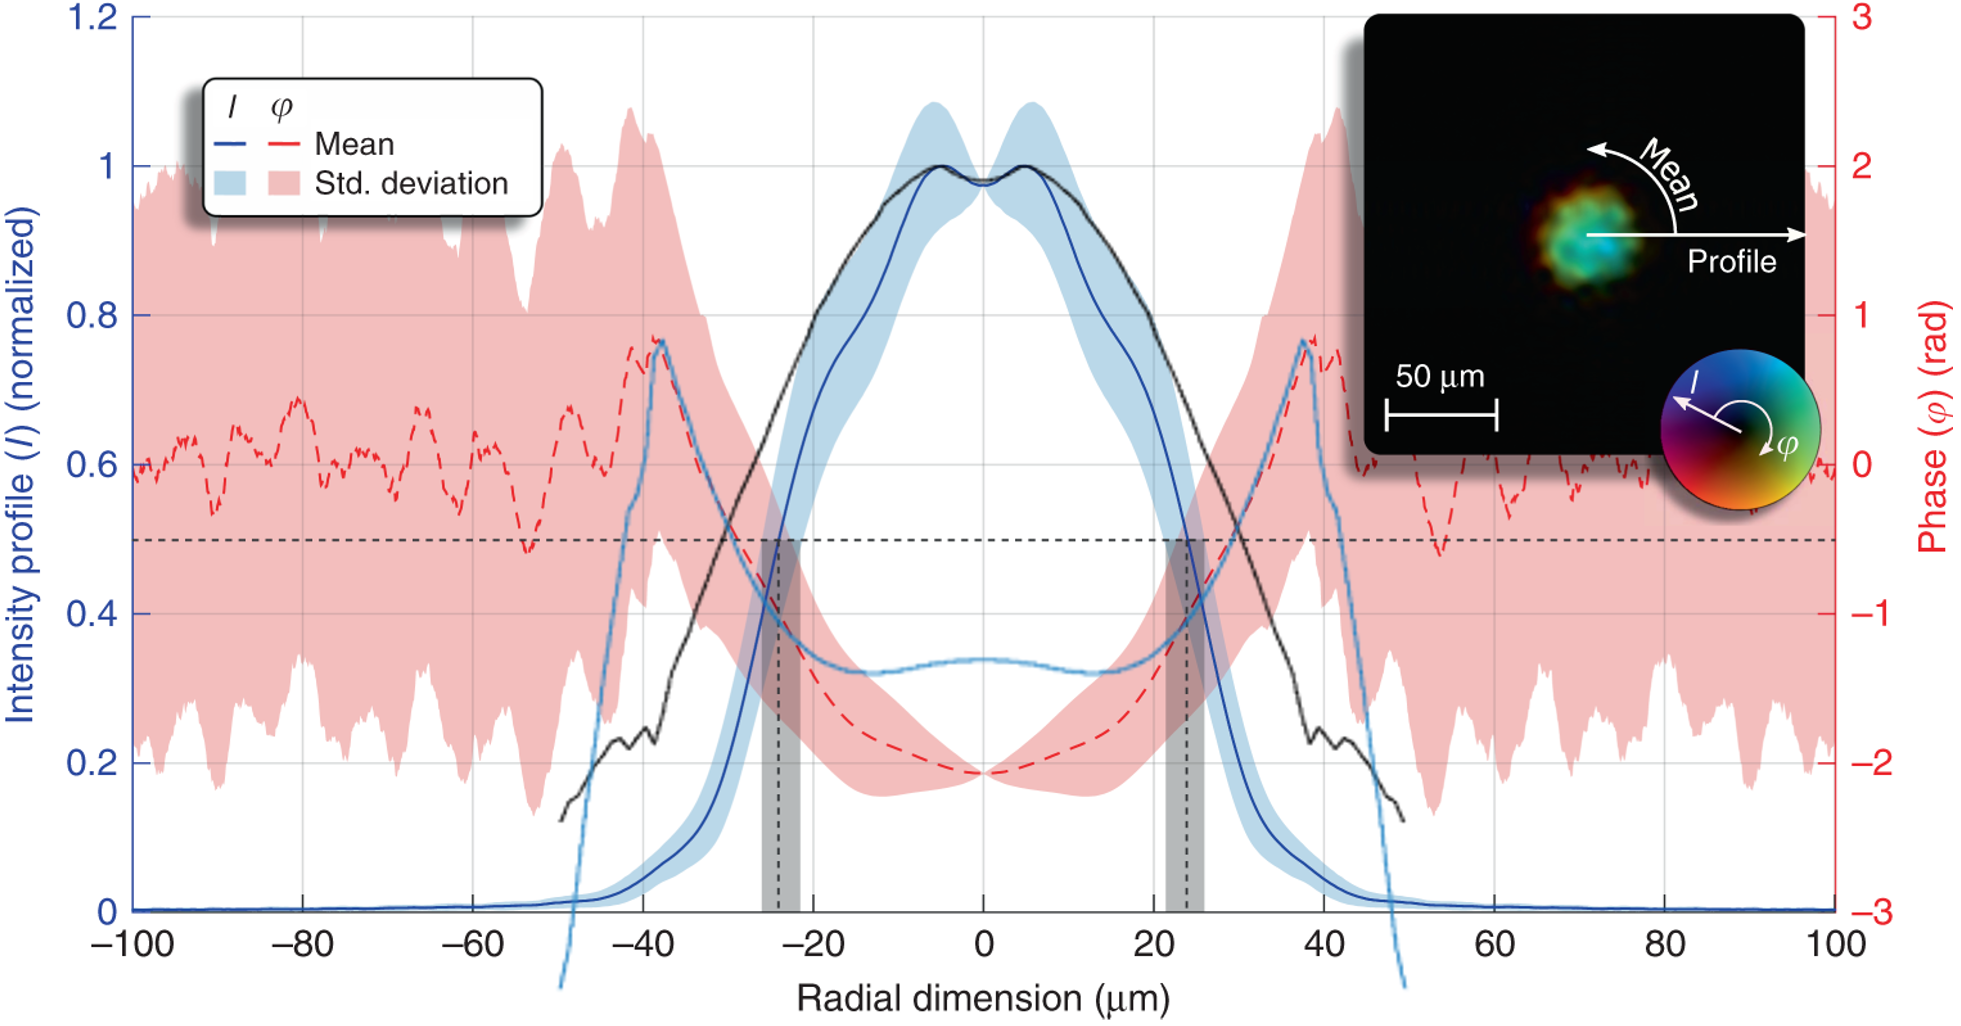
\includegraphics[width=0.74\textwidth]{Figuras/anx_cmp_55.png}
  \caption*{Comparación entre los perfiles radiales de intensidad--fase con $r_{ig,min}=\qty{15}{µm}$ y $r_{ig,max}=\qty{23}{µm}$, manteniendo los valores de los parámetros $k_{ig}=\qty{5000}{m^{-1}}$ y $z_{0ig}=\qty{4}{mm}$; y el experimento.}
\end{figure}

\begin{figure}[htbp]
  \centering
  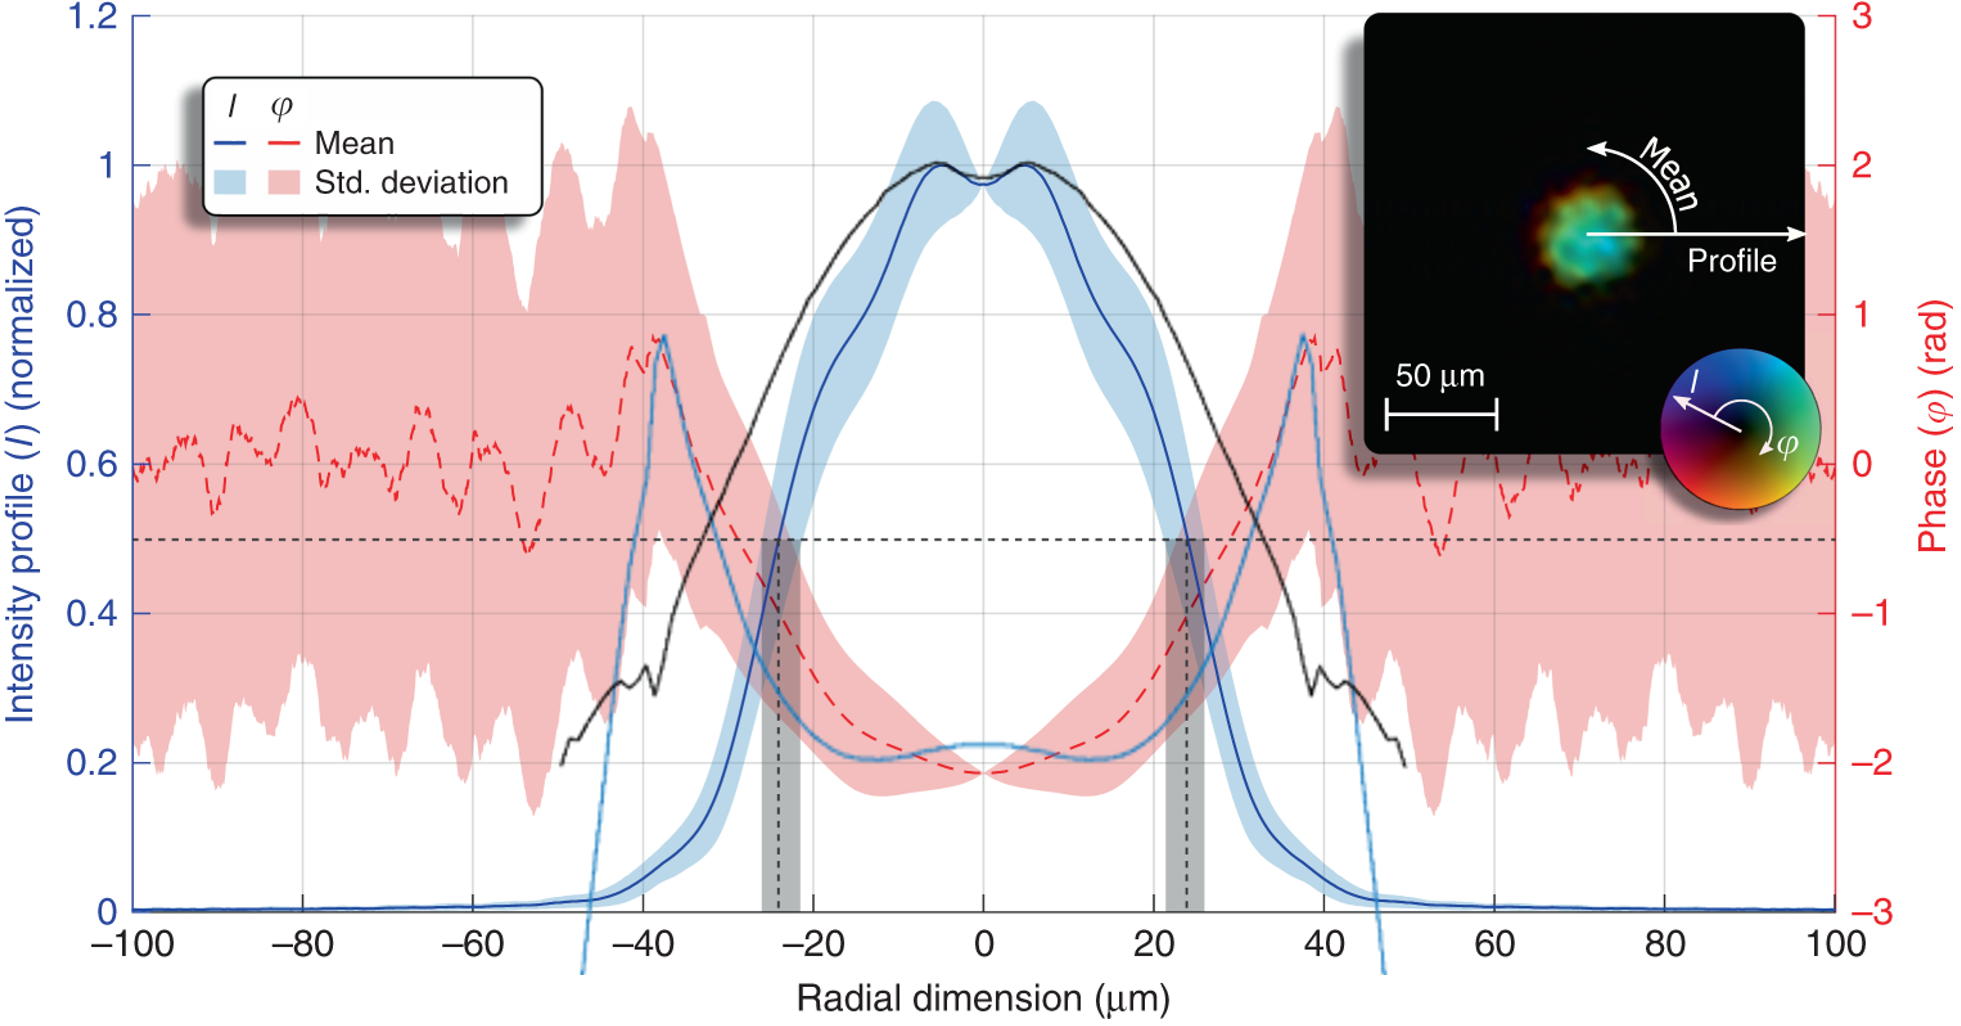
\includegraphics[width=0.7\textwidth]{Figuras/anx_cmp_56.png}
  \caption*{Comparación entre los perfiles radiales de intensidad--fase con $r_{ig,min}=\qty{15}{µm}$ y $r_{ig,max}=\qty{25}{µm}$, manteniendo los valores de los parámetros $k_{ig}=\qty{5000}{m^{-1}}$ y $z_{0ig}=\qty{4}{mm}$; y el experimento.}
\end{figure}

\newpage

\subsection*{Variando el parámetro $z_{0ig}$}

\begin{figure}[htbp!]
  \centering
  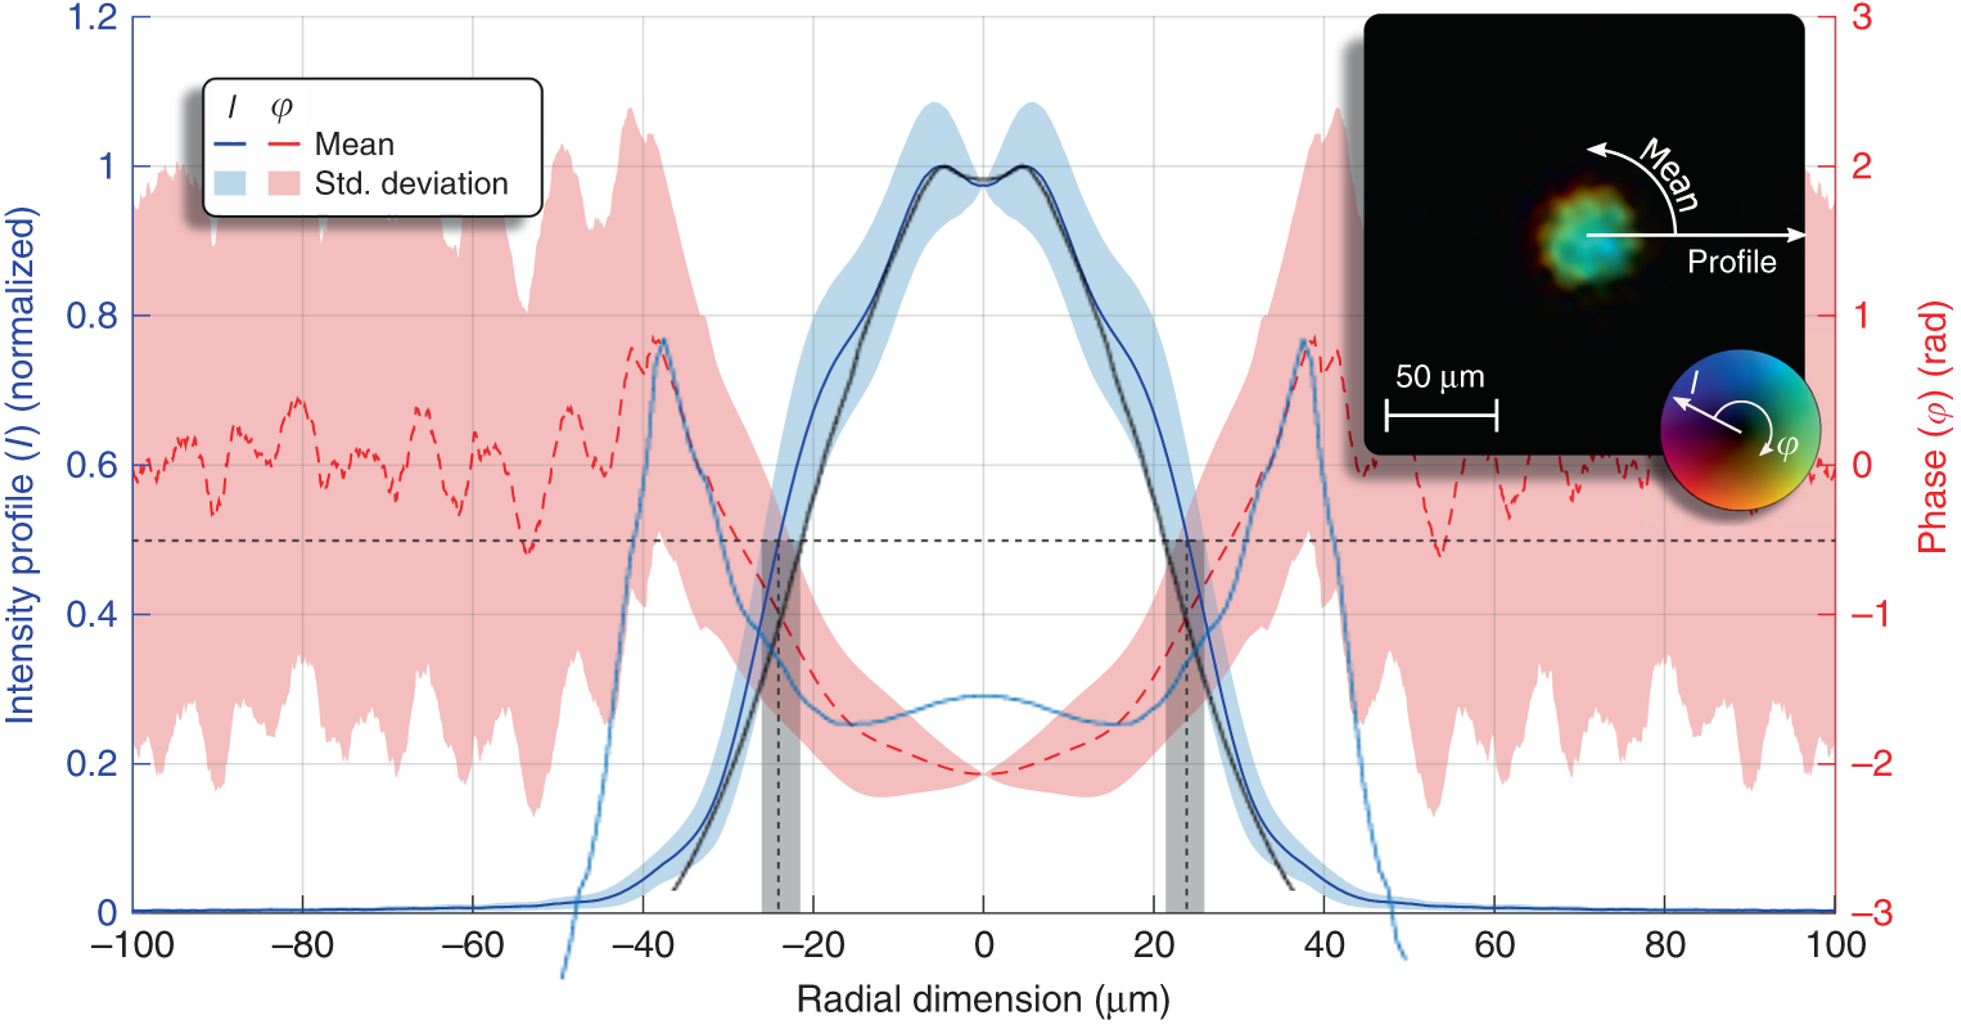
\includegraphics[width=0.74\textwidth]{Figuras/anx_cmp_61.png}
  \caption*{Comparación entre los perfiles radiales de intensidad--fase con $r_{ig,min}=r_{ig,max}=\qty{15}{µm}$, manteniendo los valores de los parámetros $k_{ig}=\qty{5000}{m^{-1}}$ y $z_{0ig}=\qty{2}{mm}$; y el experimento.}
\end{figure}

\begin{figure}[htbp!]
  \centering
  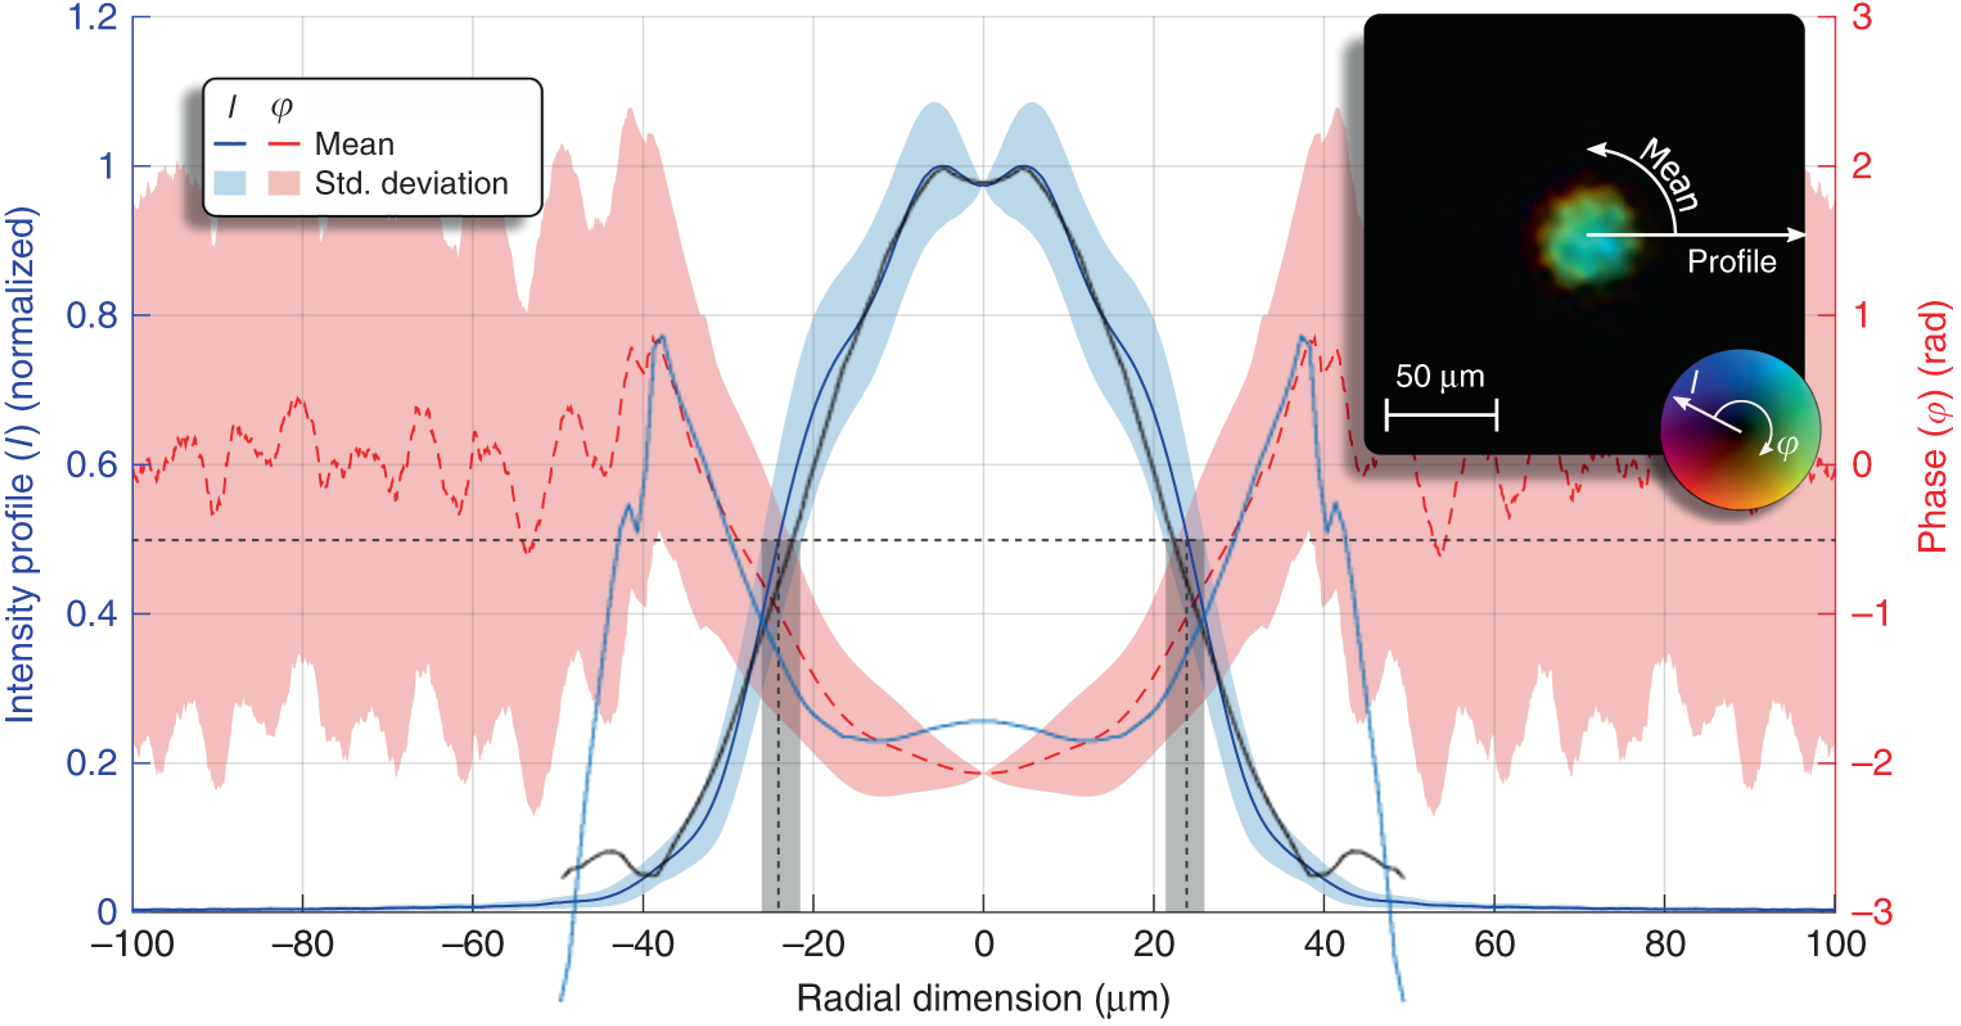
\includegraphics[width=0.74\textwidth]{Figuras/anx_cmp_62.png}
  \caption*{Comparación entre los perfiles radiales de intensidad--fase con $r_{ig,min}=\qty{15}{µm}$ y $r_{ig,max}=\qty{25}{µm}$, manteniendo los valores de los parámetros $k_{ig}=\qty{5000}{m^{-1}}$ y $z_{0ig}=\qty{2}{mm}$; y el experimento.}
\end{figure}

\begin{figure}[htbp]
  \centering
  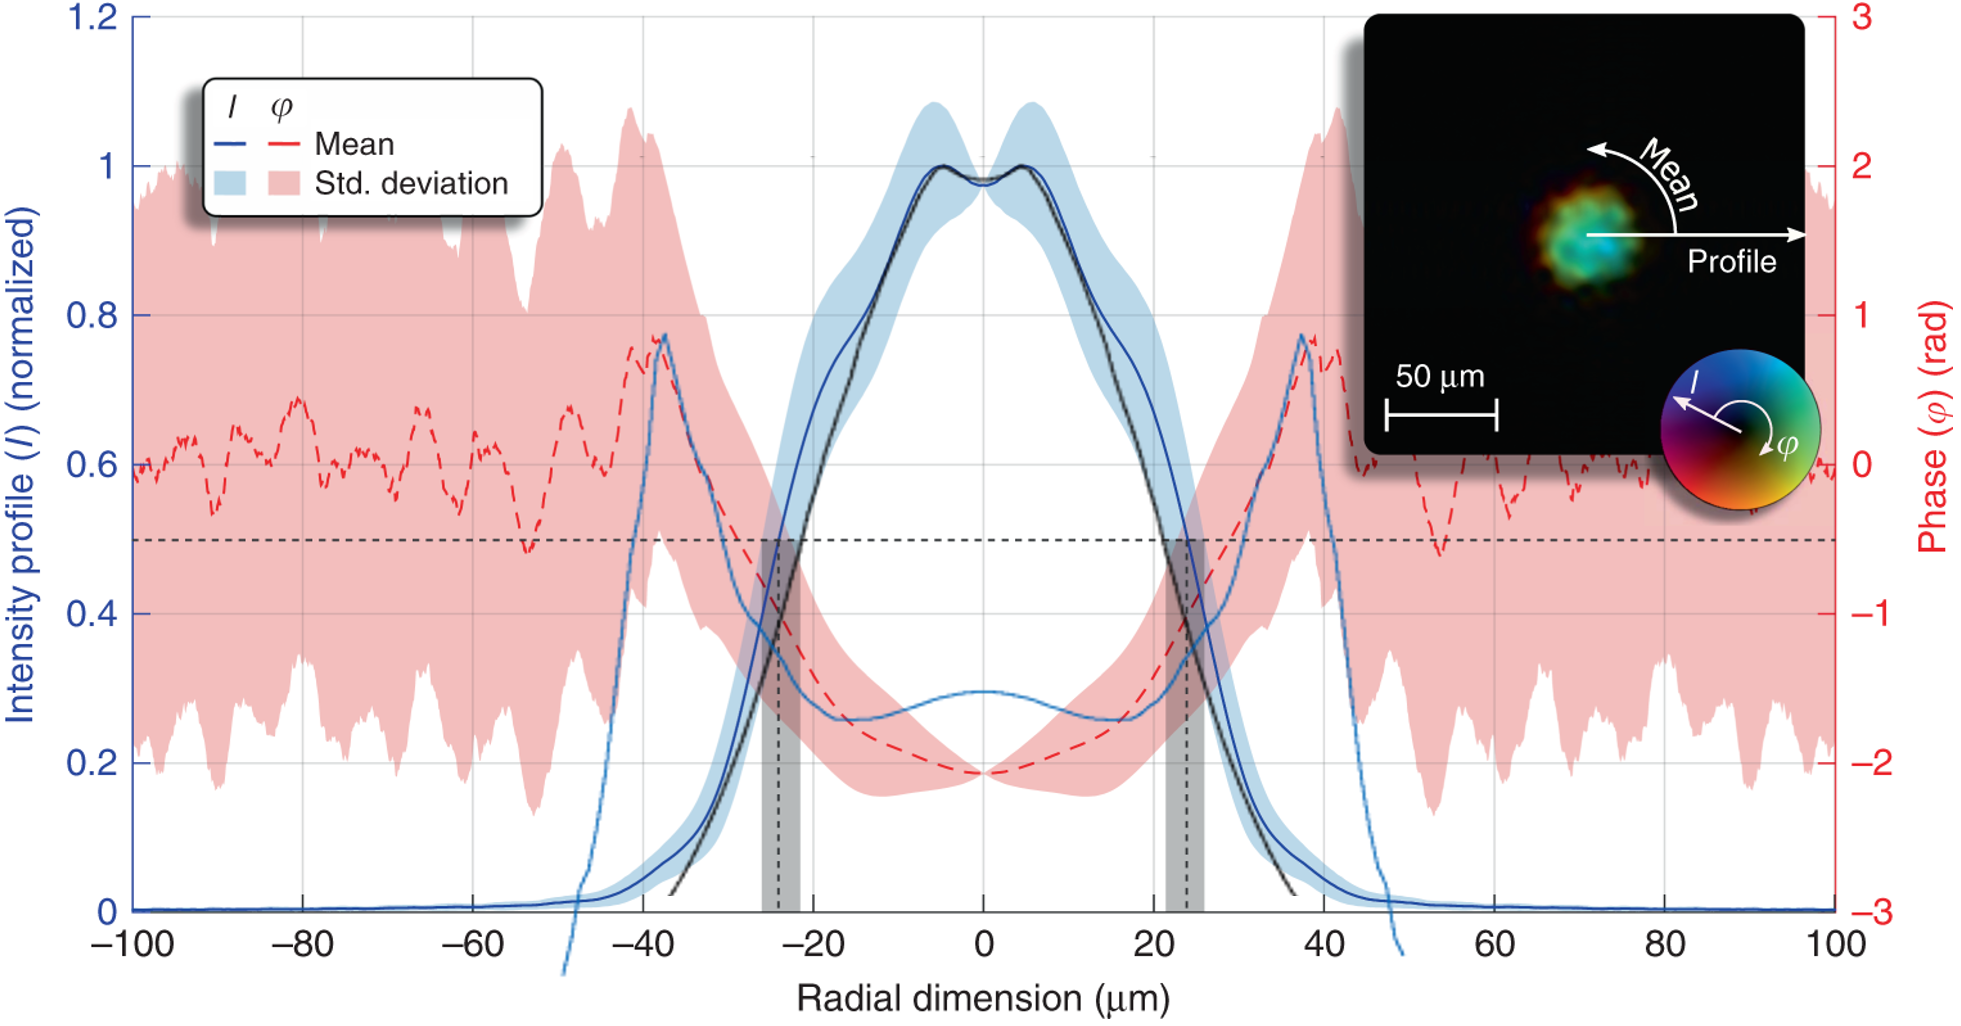
\includegraphics[width=0.74\textwidth]{Figuras/anx_cmp_63.png}
  \caption*{Comparación entre los perfiles radiales de intensidad--fase con $r_{ig,min}=r_{ig,max}=\qty{15}{µm}$, manteniendo los valores de los parámetros $k_{ig}=\qty{5000}{m^{-1}}$ y $z_{0ig}=\qty{2.5}{mm}$; y el experimento.}
\end{figure}

\begin{figure}[htbp]
  \centering
  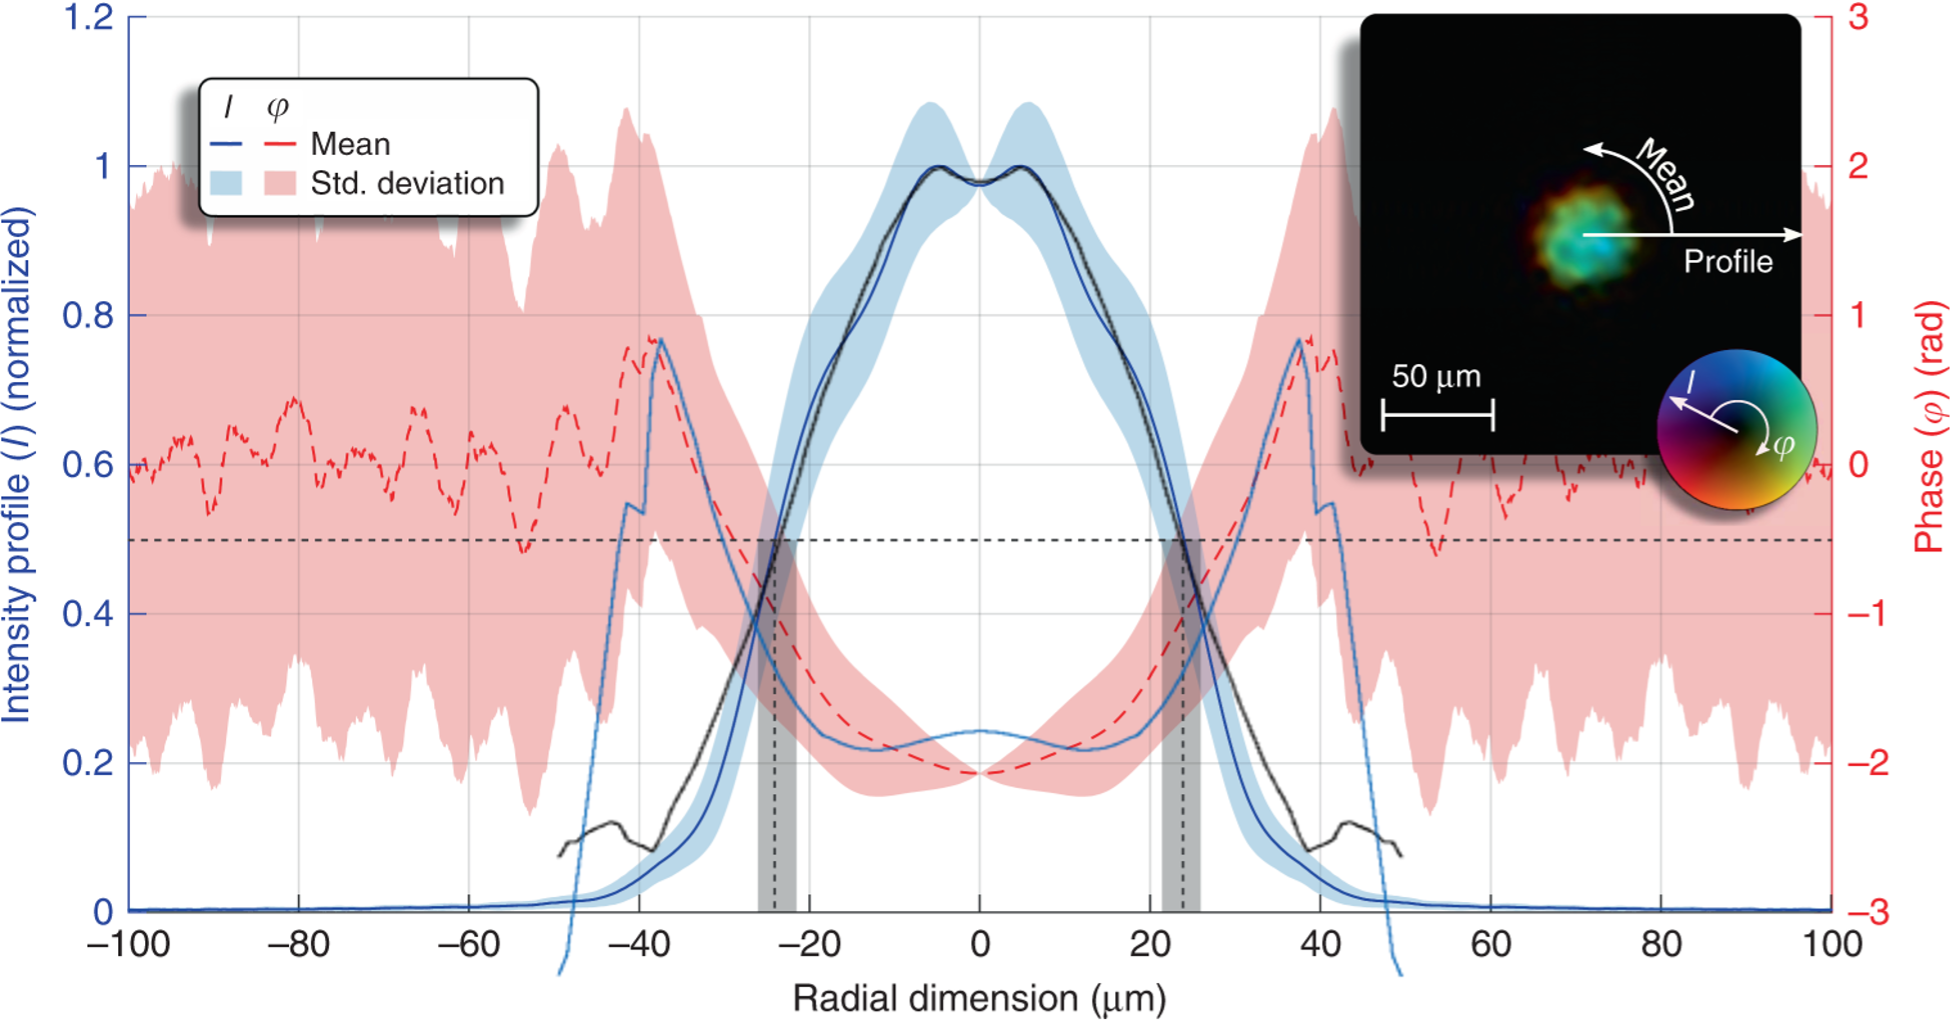
\includegraphics[width=0.74\textwidth]{Figuras/anx_cmp_64.png}
  \caption*{Comparación entre los perfiles radiales de intensidad--fase con $r_{ig,min}=\qty{15}{µm}$ y $r_{ig,max}=\qty{25}{µm}$, manteniendo los valores de los parámetros $k_{ig}=\qty{5000}{m^{-1}}$ y $z_{0ig}=\qty{2.5}{mm}$; y el experimento.}
\end{figure}

\begin{figure}[htbp]
  \centering
  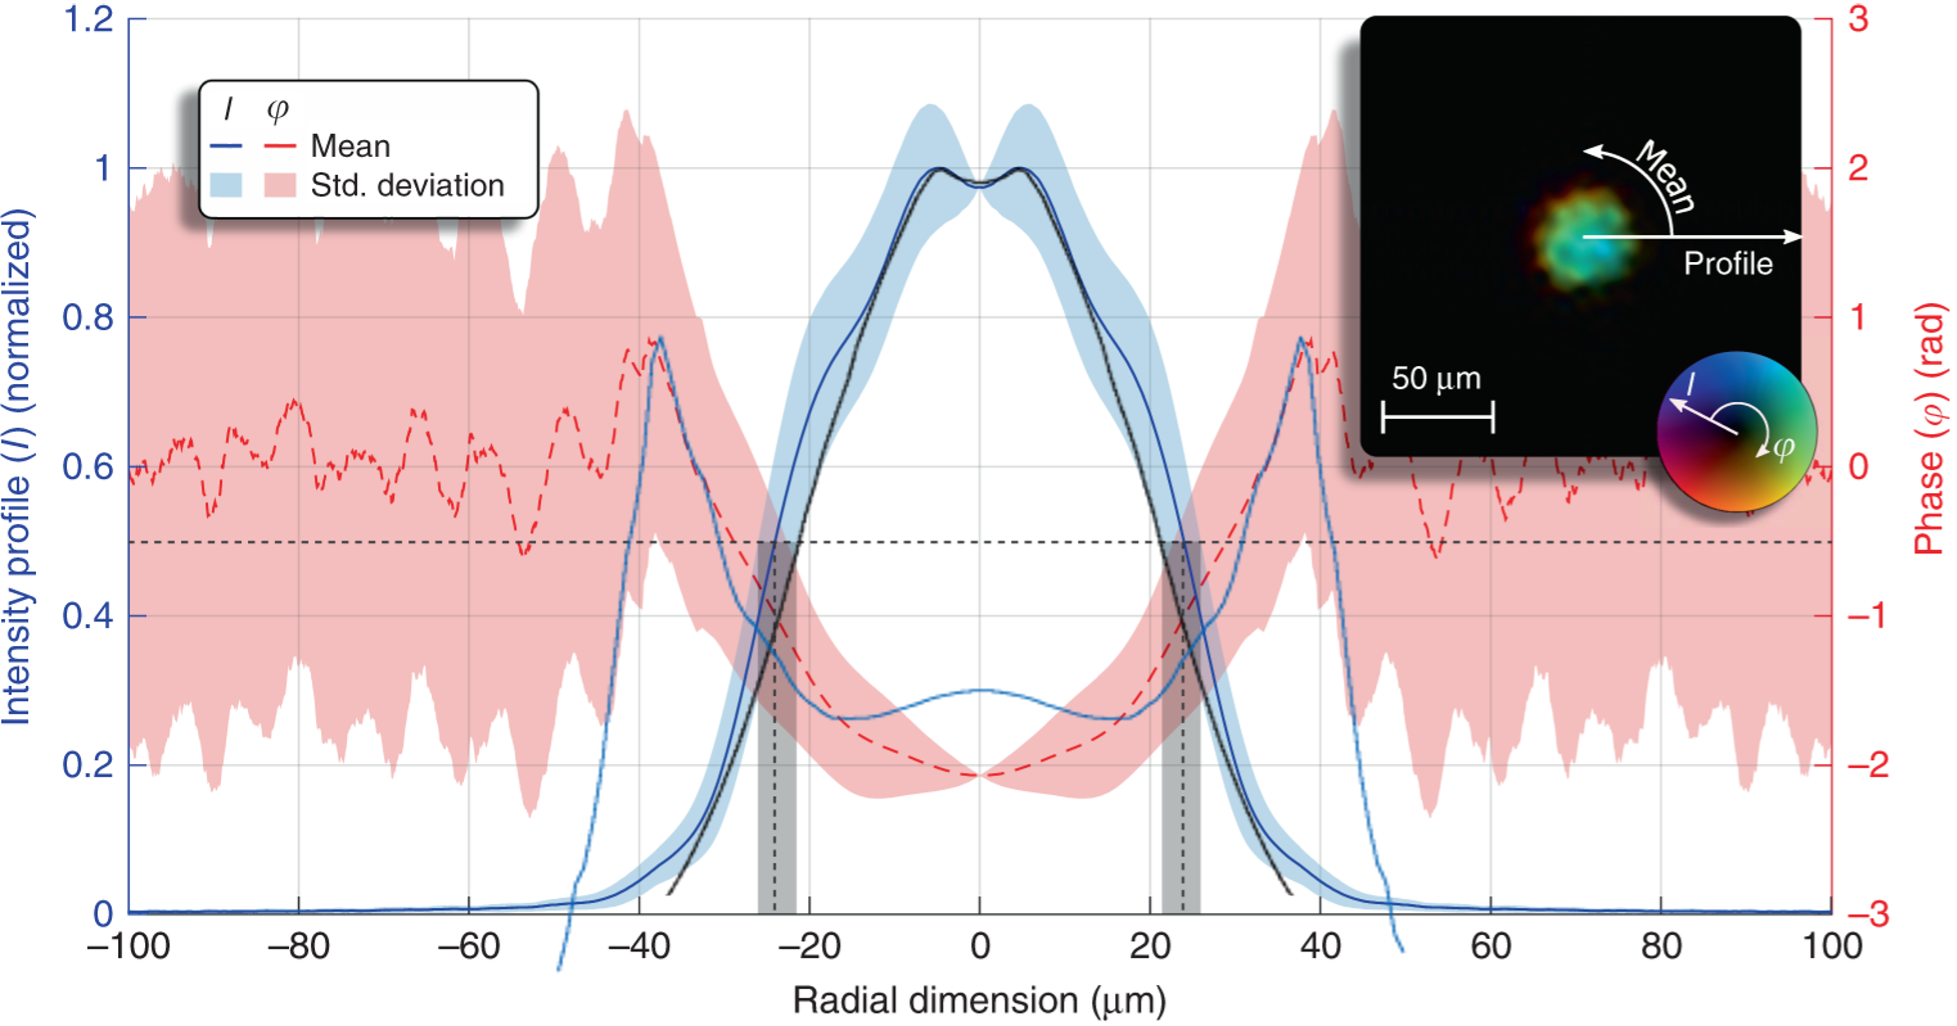
\includegraphics[width=0.74\textwidth]{Figuras/anx_cmp_65.png}
  \caption*{Comparación entre los perfiles radiales de intensidad--fase con $r_{ig,min}=r_{ig,max}=\qty{15}{µm}$, manteniendo los valores de los parámetros $k_{ig}=\qty{5000}{m^{-1}}$ y $z_{0ig}=\qty{3}{mm}$; y el experimento.}
\end{figure}

\begin{figure}[htbp]
  \centering
  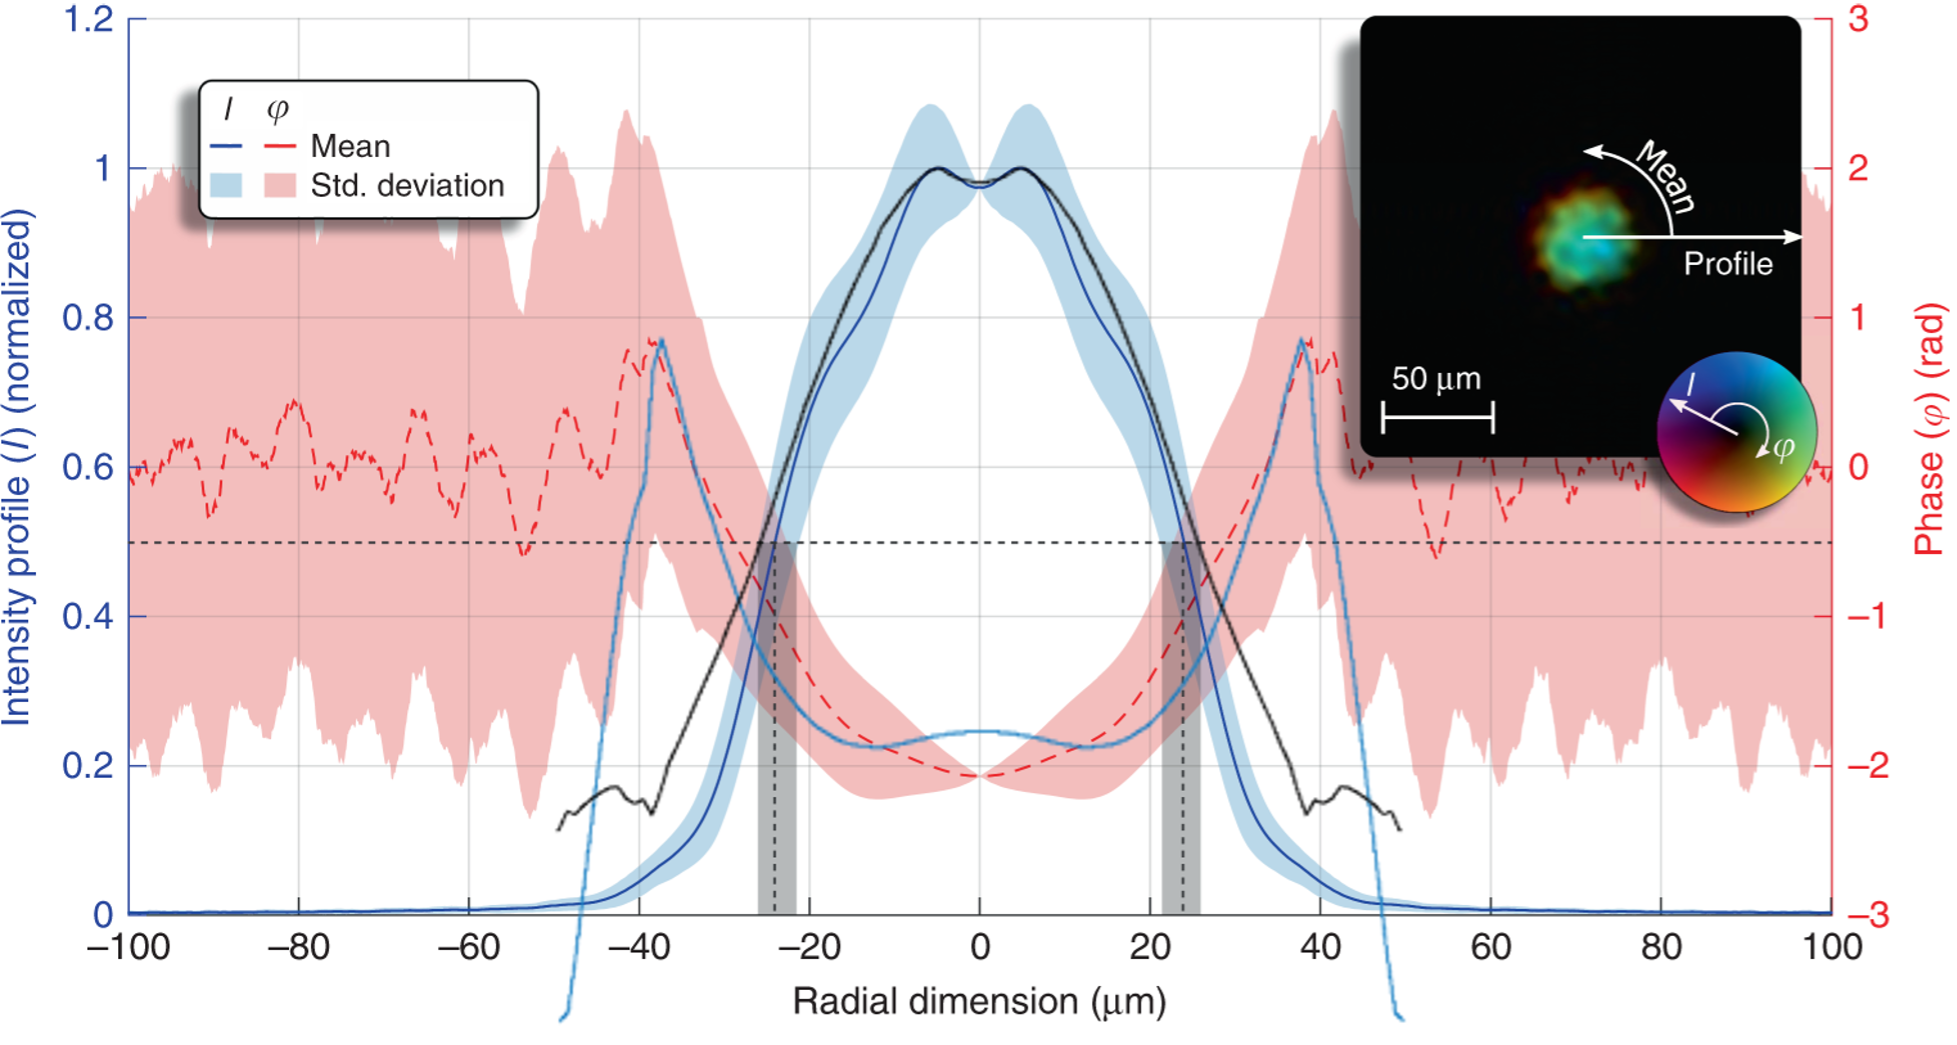
\includegraphics[width=0.74\textwidth]{Figuras/anx_cmp_66.png}
  \caption*{Comparación entre los perfiles radiales de intensidad--fase con $r_{ig,min}=\qty{15}{µm}$ y $r_{ig,max}=\qty{25}{µm}$, manteniendo los valores de los parámetros $k_{ig}=\qty{5000}{m^{-1}}$ y $z_{0ig}=\qty{3}{mm}$; y el experimento.}
\end{figure}

\begin{figure}[htbp]
  \centering
  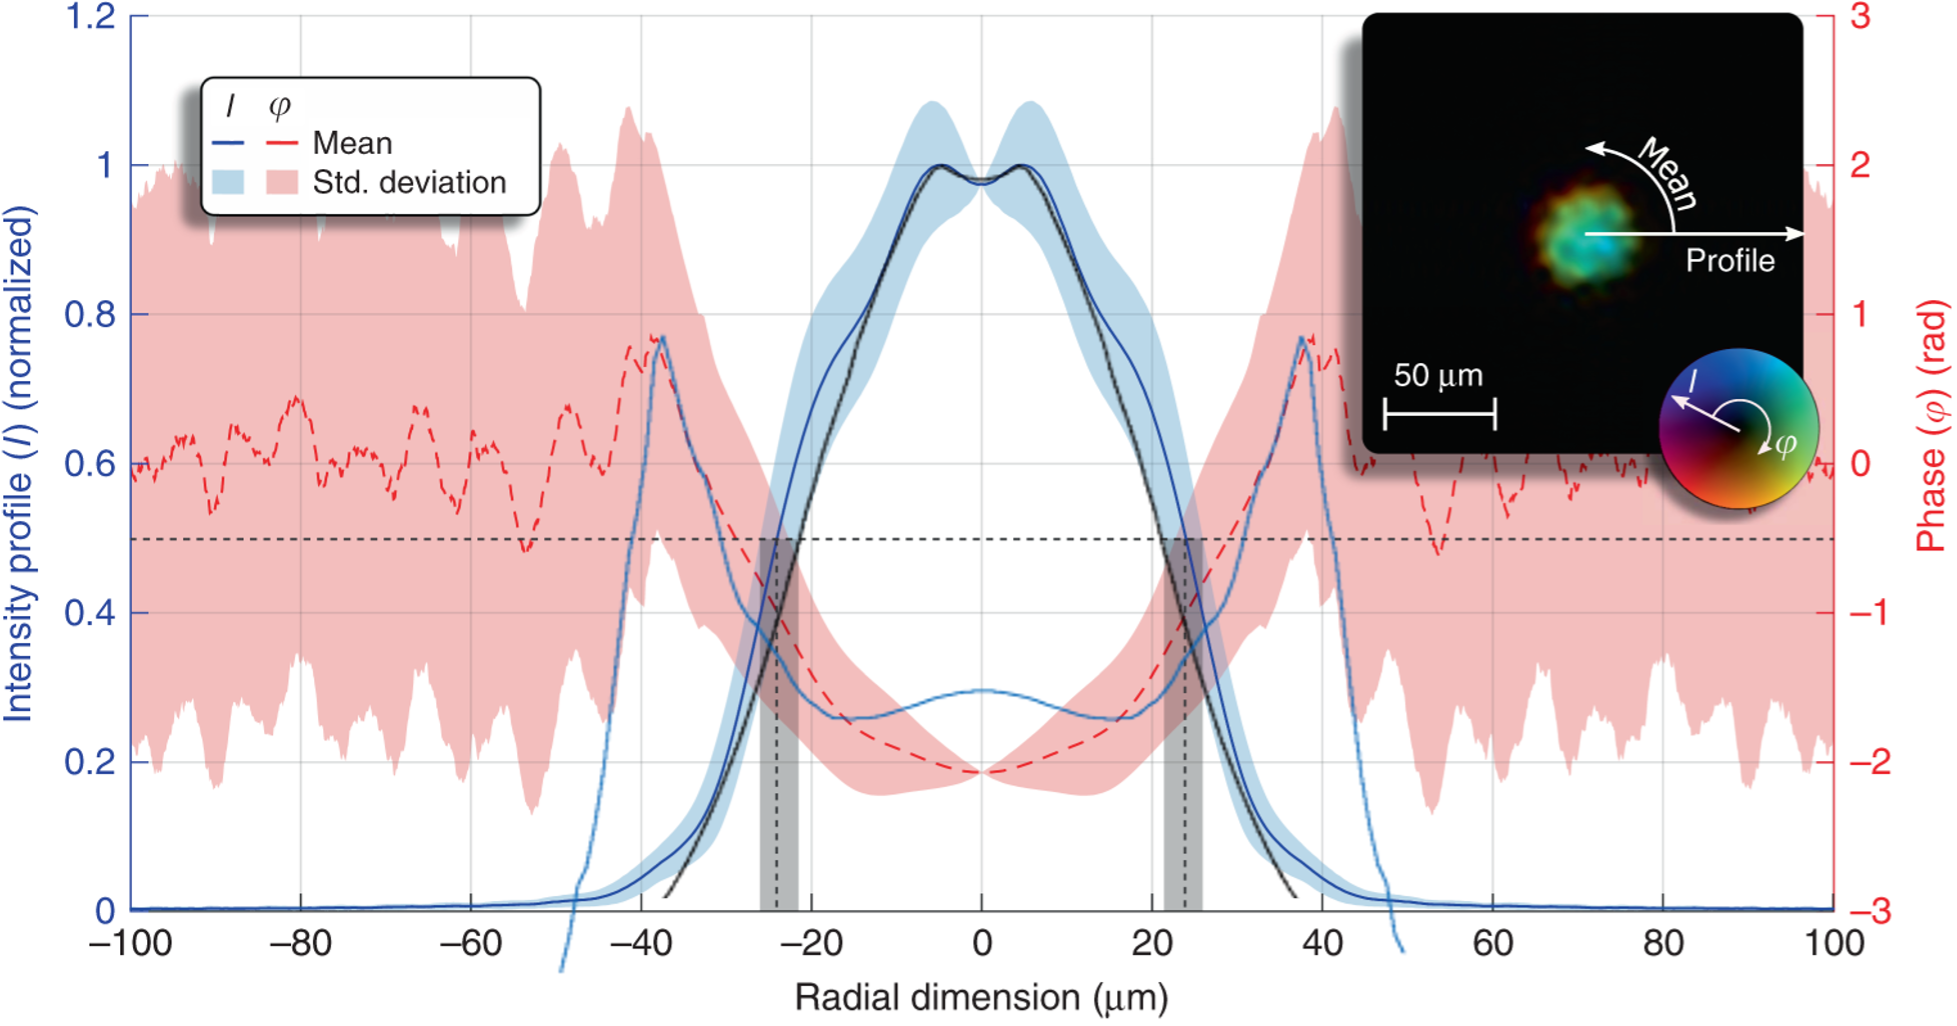
\includegraphics[width=0.74\textwidth]{Figuras/anx_cmp_67.png}
  \caption*{Comparación entre los perfiles radiales de intensidad--fase con $r_{ig,min}=r_{ig,max}=\qty{15}{µm}$, manteniendo los valores de los parámetros $k_{ig}=\qty{5000}{m^{-1}}$ y $z_{0ig}=\qty{3.5}{mm}$; y el experimento.}
\end{figure}

\begin{figure}[htbp]
  \centering
  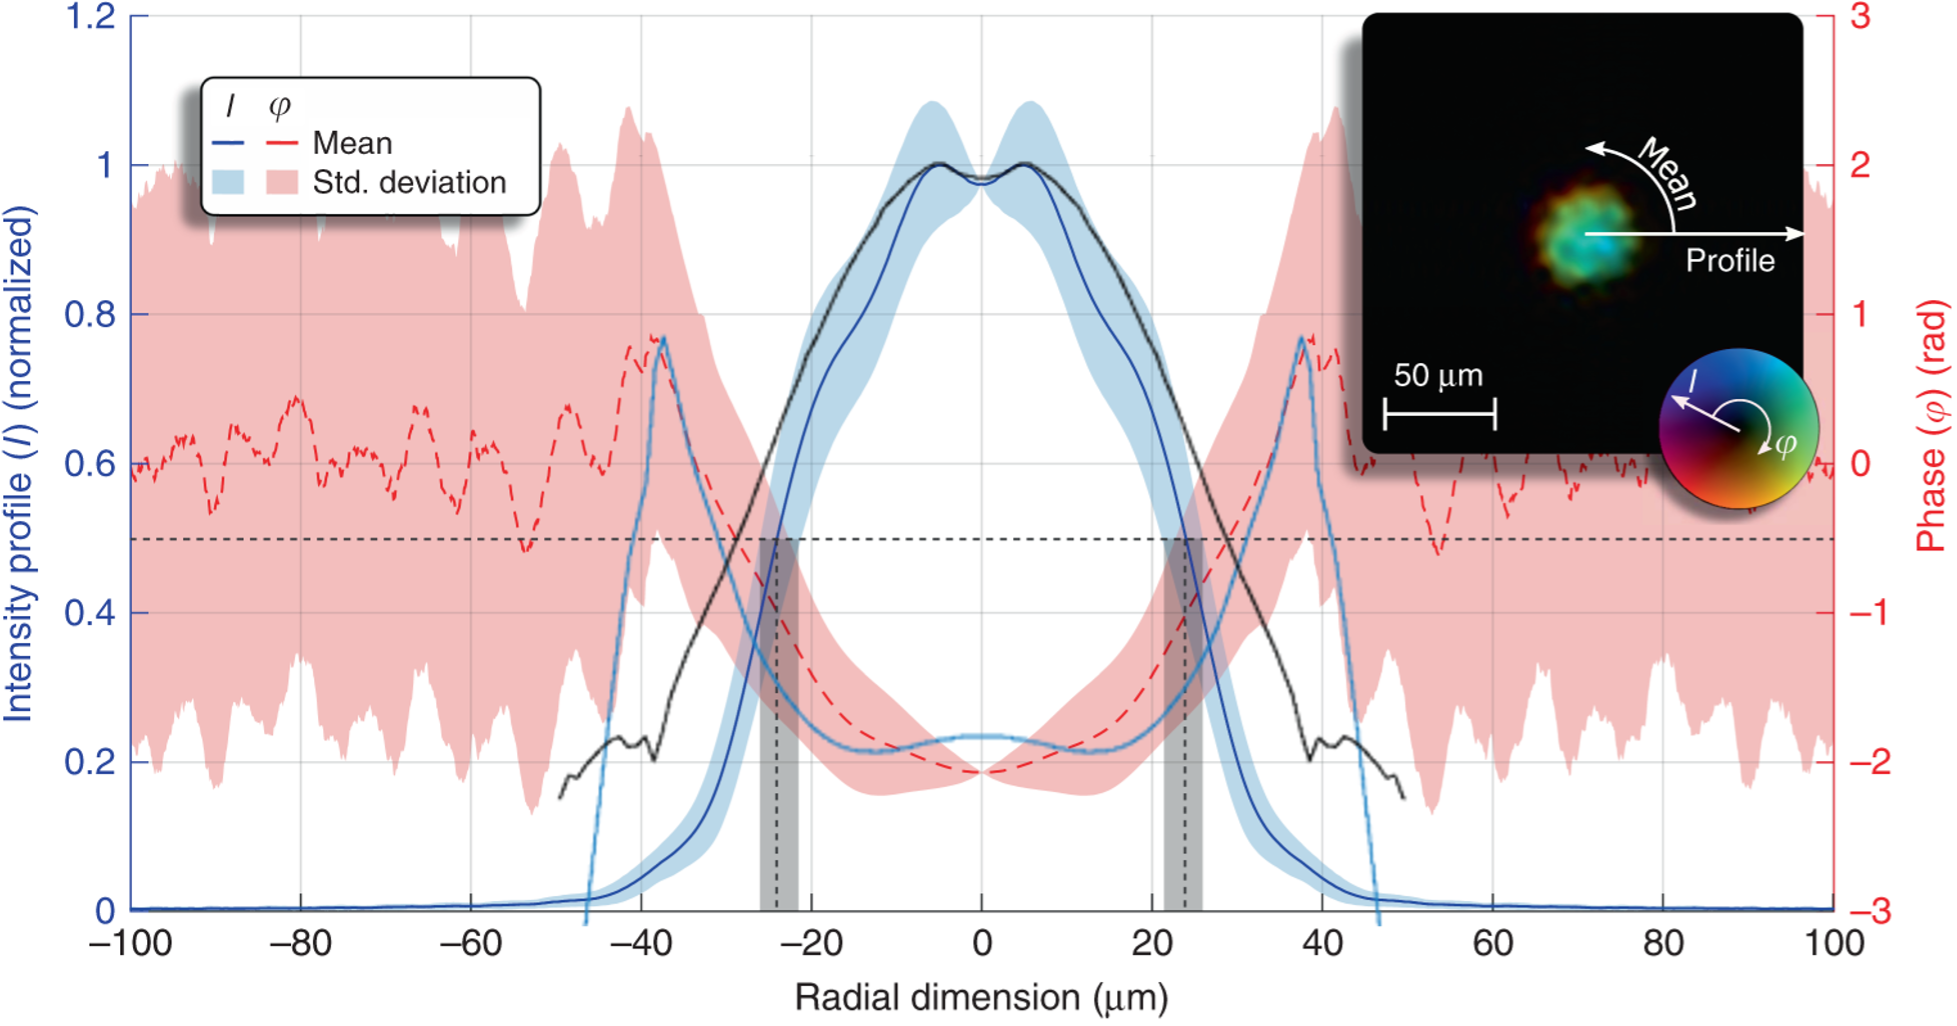
\includegraphics[width=0.74\textwidth]{Figuras/anx_cmp_68.png}
  \caption*{Comparación entre los perfiles radiales de intensidad--fase con $r_{ig,min}=\qty{15}{µm}$ y $r_{ig,max}=\qty{25}{µm}$, manteniendo los valores de los parámetros $k_{ig}=\qty{5000}{m^{-1}}$ y $z_{0ig}=\qty{3.5}{mm}$; y el experimento.}
\end{figure}

\newpage

\begin{figure}[htbp]
  \centering
  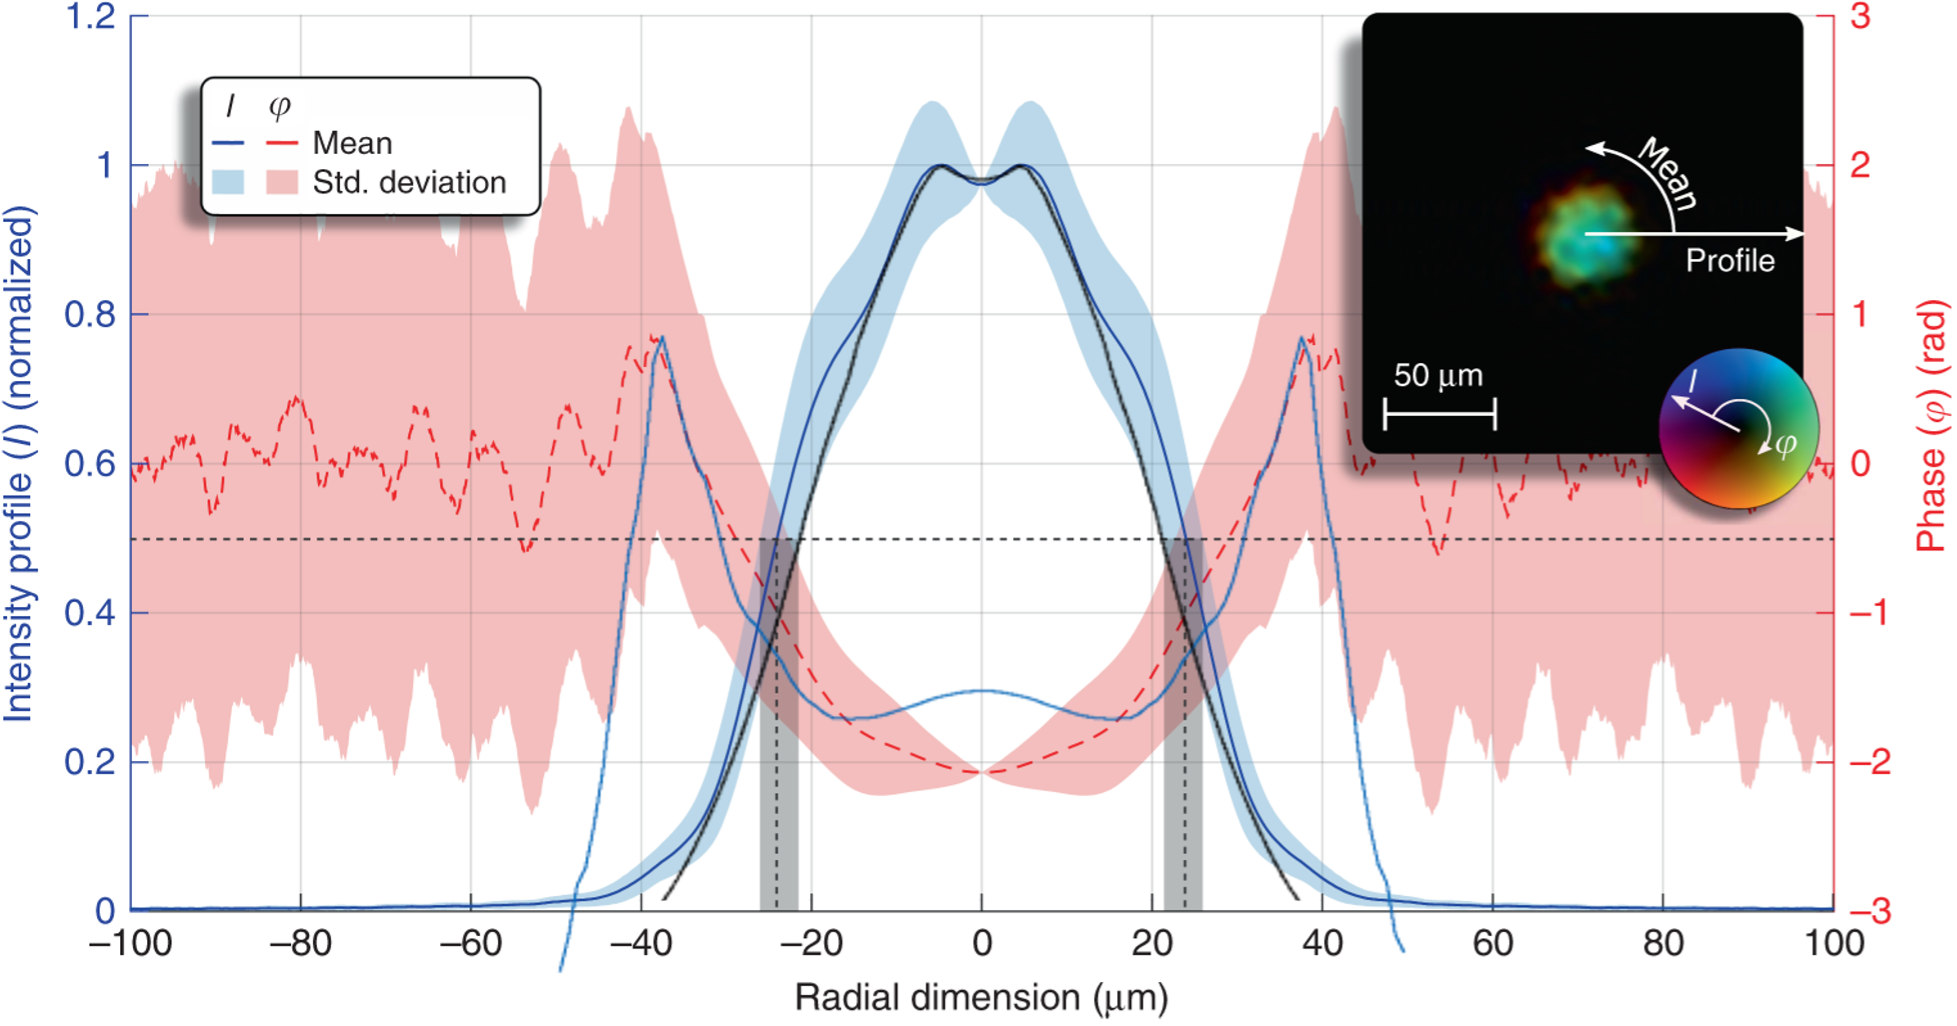
\includegraphics[width=0.7\textwidth]{Figuras/anx_cmp_69.png}
  \caption*{Comparación entre los perfiles radiales de intensidad--fase con $r_{ig,min}=r_{ig,max}=\qty{15}{µm}$, manteniendo los valores de los parámetros $k_{ig}=\qty{5000}{m^{-1}}$ y $z_{0ig}=\qty{4}{mm}$; y el experimento.}
\end{figure}

\begin{figure}[htbp]
  \centering
  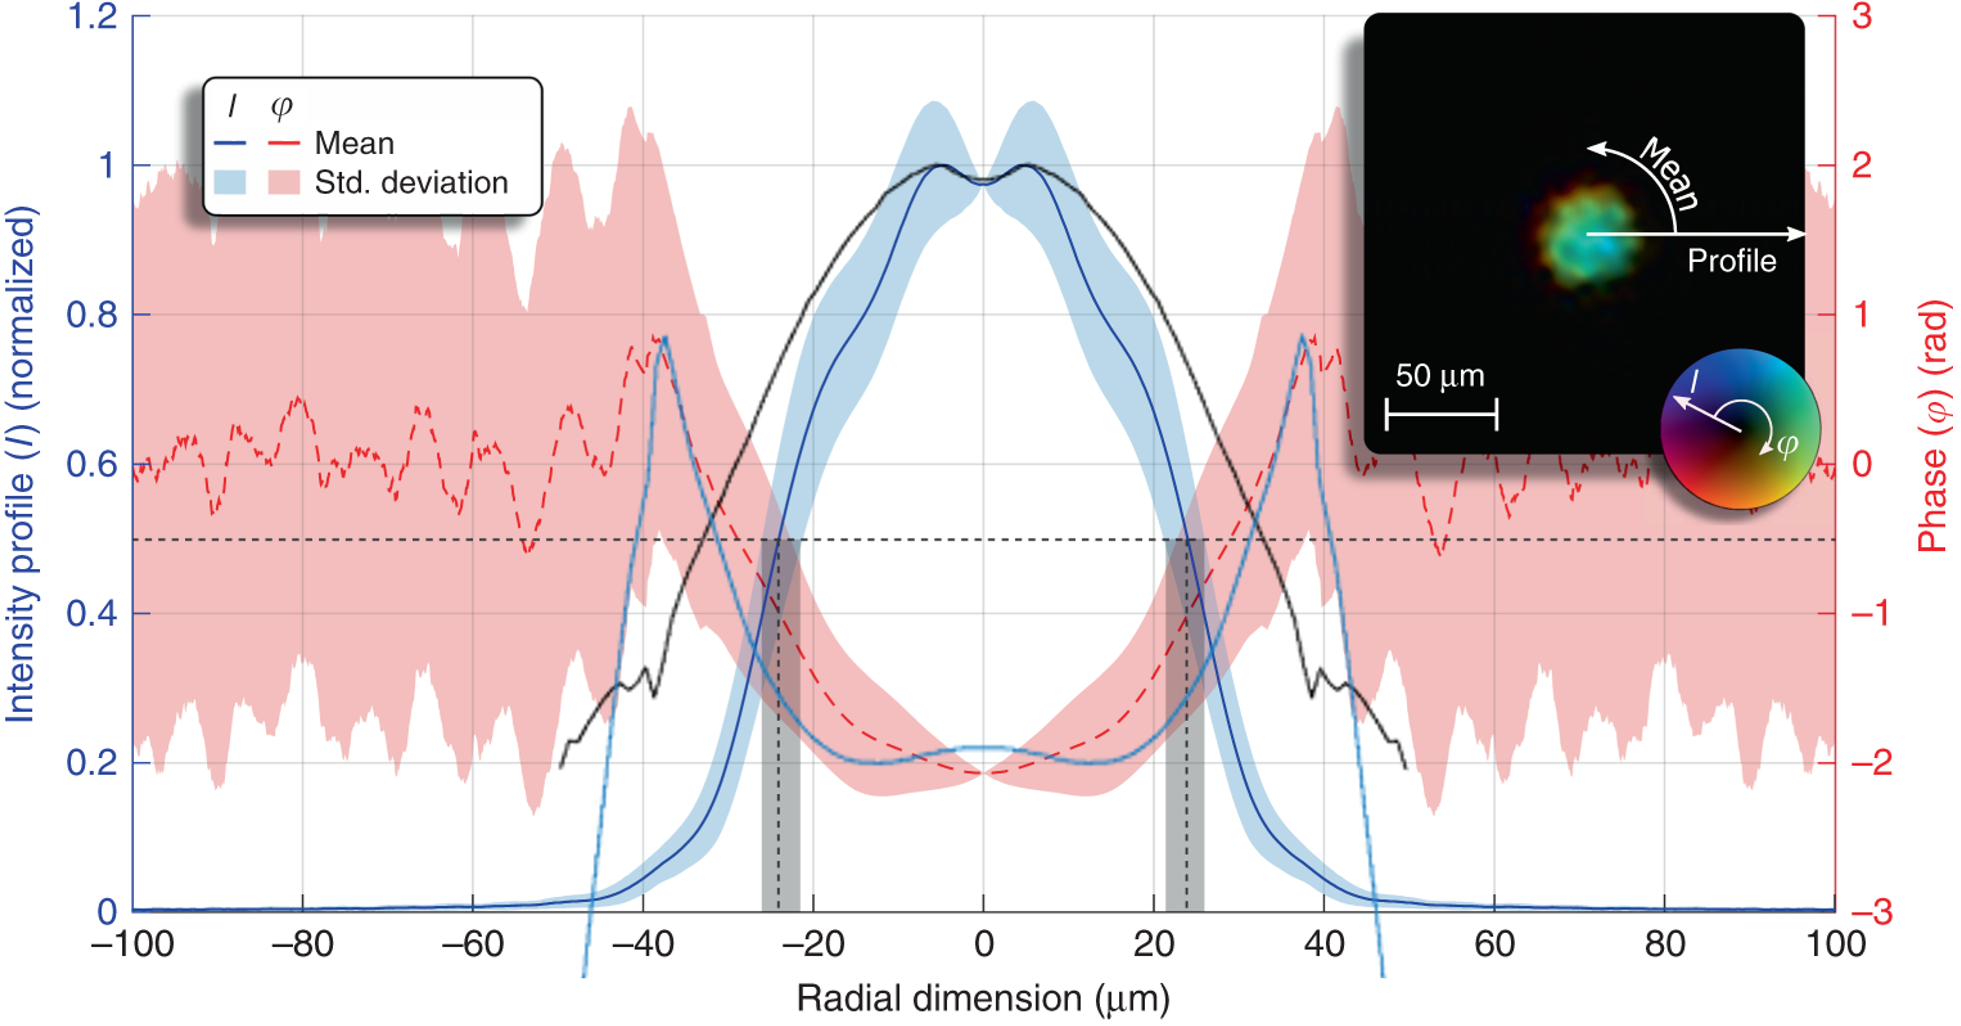
\includegraphics[width=0.7\textwidth]{Figuras/anx_cmp_60.png}
  \caption*{Comparación entre los perfiles radiales de intensidad--fase con $r_{ig,min}=\qty{15}{µm}$ y $r_{ig,max}=\qty{25}{µm}$, manteniendo los valores de los parámetros $k_{ig}=\qty{5000}{m^{-1}}$ y $z_{0ig}=\qty{4}{mm}$; y el experimento.}
\end{figure}

\subsection*{Variando el parámetro $k_{ig}$}

\begin{figure}[htbp!]
  \centering
  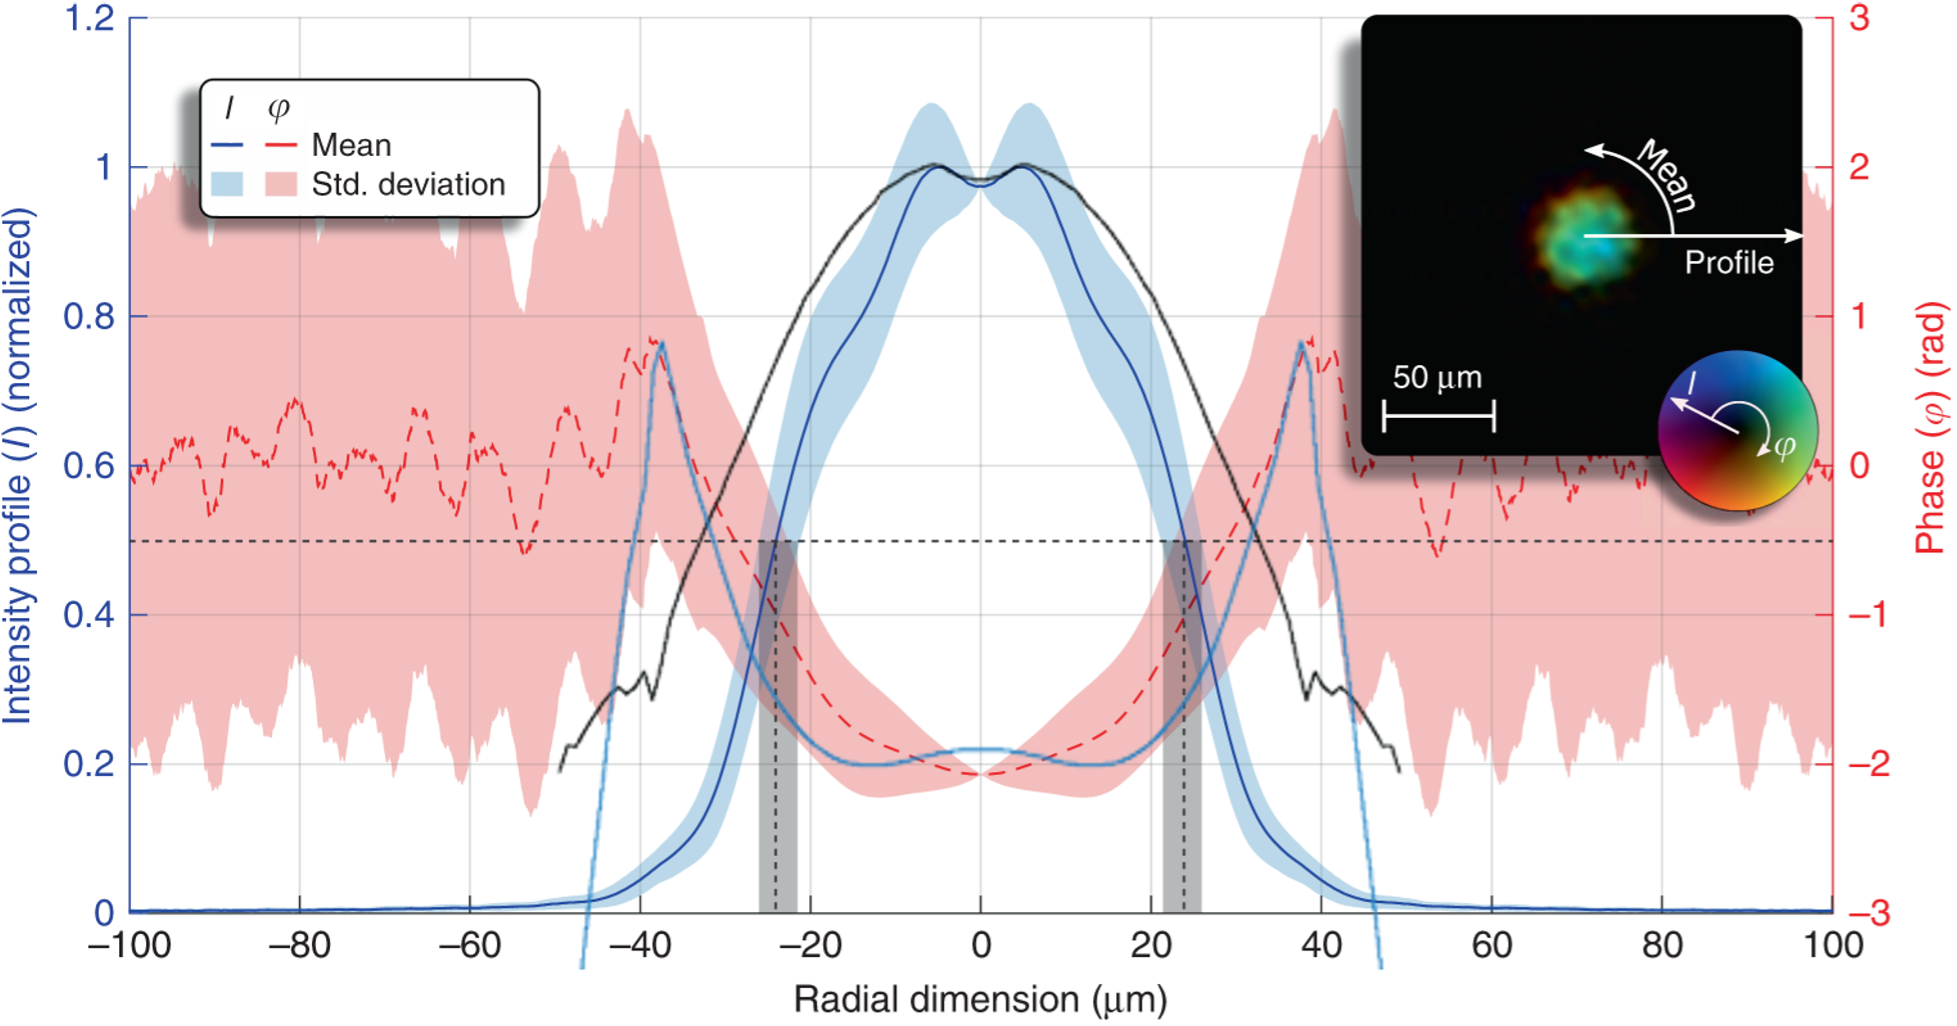
\includegraphics[width=0.7\textwidth]{Figuras/anx_cmp_71.png}
  \caption*{Comparación entre los perfiles radiales de intensidad--fase con $k_{ig}=\qty{3500}{m^{-1}}$, manteniendo los valores de los parámetros $r_{ig,min}=\qty{15}{µm}$, $r_{ig,max}=\qty{25}{µm}$ y $z_{0ig}=\qty{4}{mm}$; y el experimento.}
\end{figure}

\begin{figure}[htbp]
  \centering
  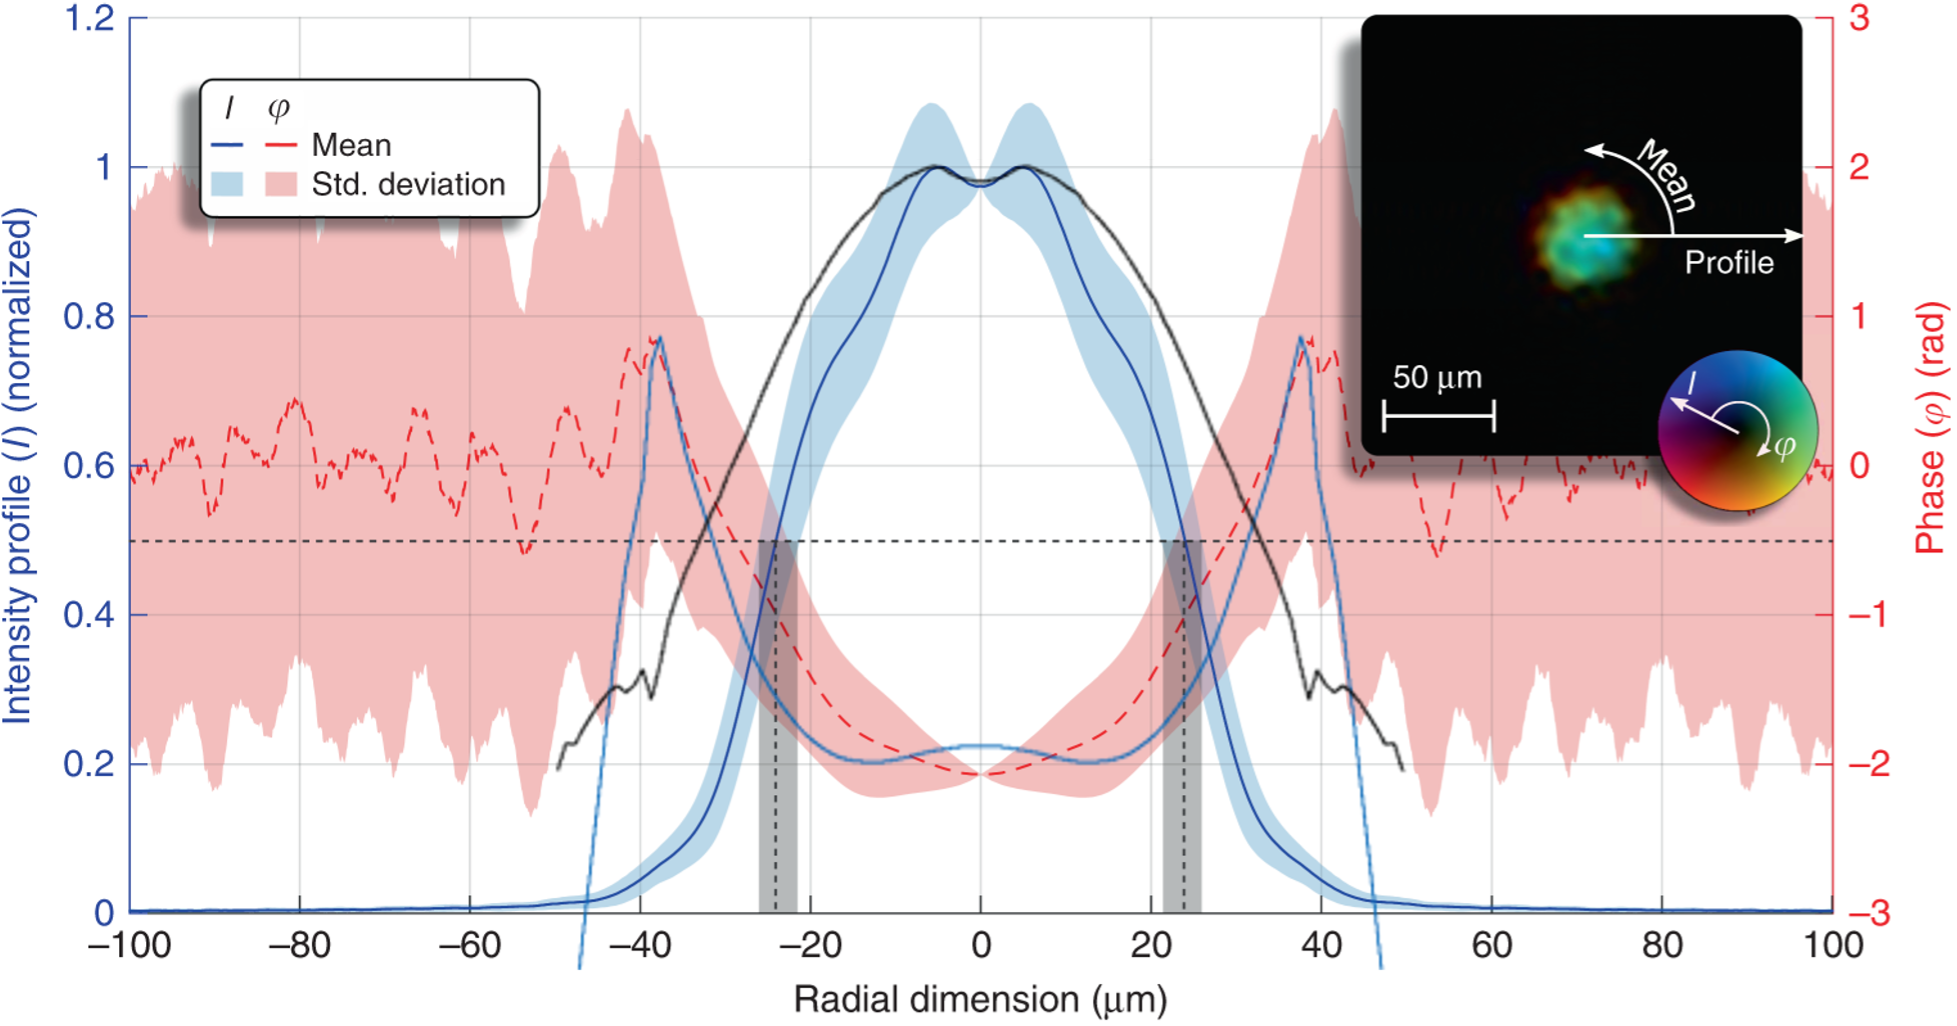
\includegraphics[width=0.7\textwidth]{Figuras/anx_cmp_72.png}
  \caption*{Comparación entre los perfiles radiales de intensidad--fase con $k_{ig}=\qty{4000}{m^{-1}}$, manteniendo los valores de los parámetros $r_{ig,min}=\qty{15}{µm}$, $r_{ig,max}=\qty{25}{µm}$ y $z_{0ig}=\qty{4}{mm}$; y el experimento.}
\end{figure}

\begin{figure}[htbp]
  \centering
  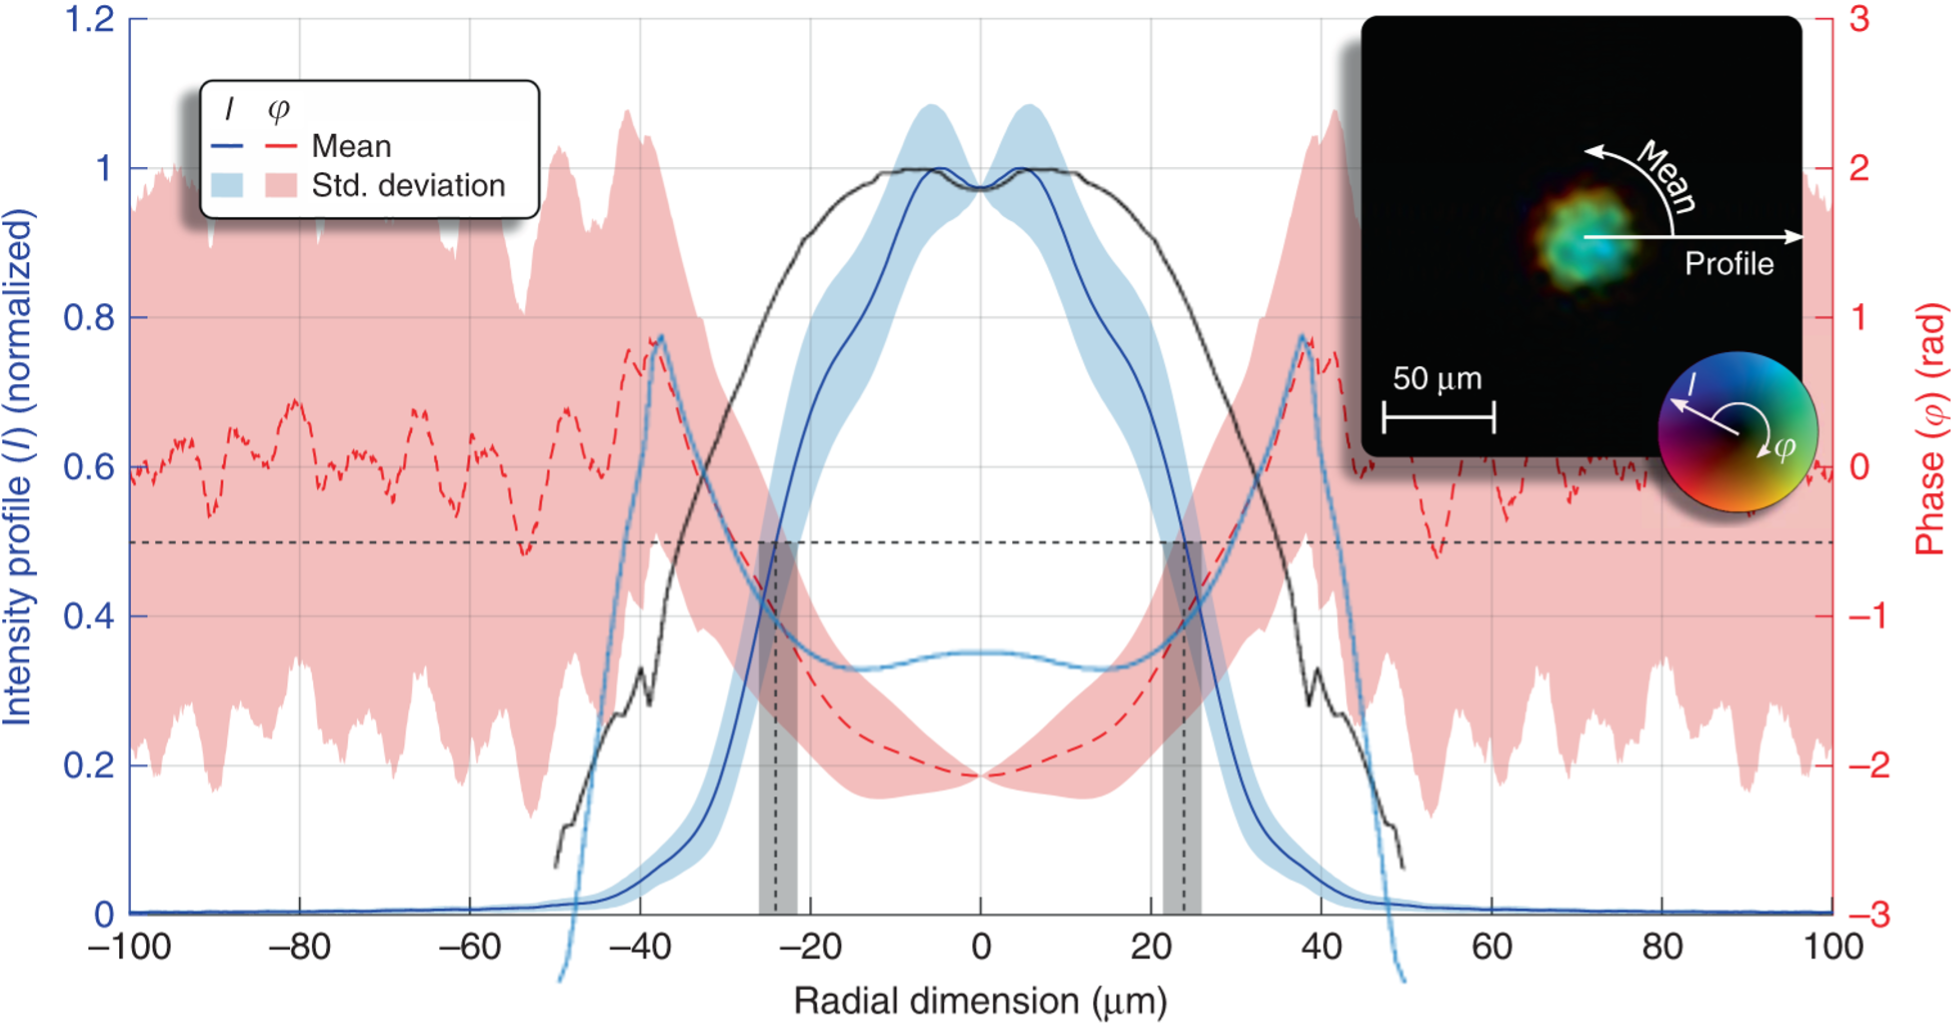
\includegraphics[width=0.7\textwidth]{Figuras/anx_cmp_73.png}
  \caption*{Comparación entre los perfiles radiales de intensidad--fase con $k_{ig}=\qty{4500}{m^{-1}}$, manteniendo los valores de los parámetros $r_{ig,min}=\qty{15}{µm}$, $r_{ig,max}=\qty{25}{µm}$ y $z_{0ig}=\qty{4}{mm}$; y el experimento.}
\end{figure}

\begin{figure}[htbp]
  \centering
  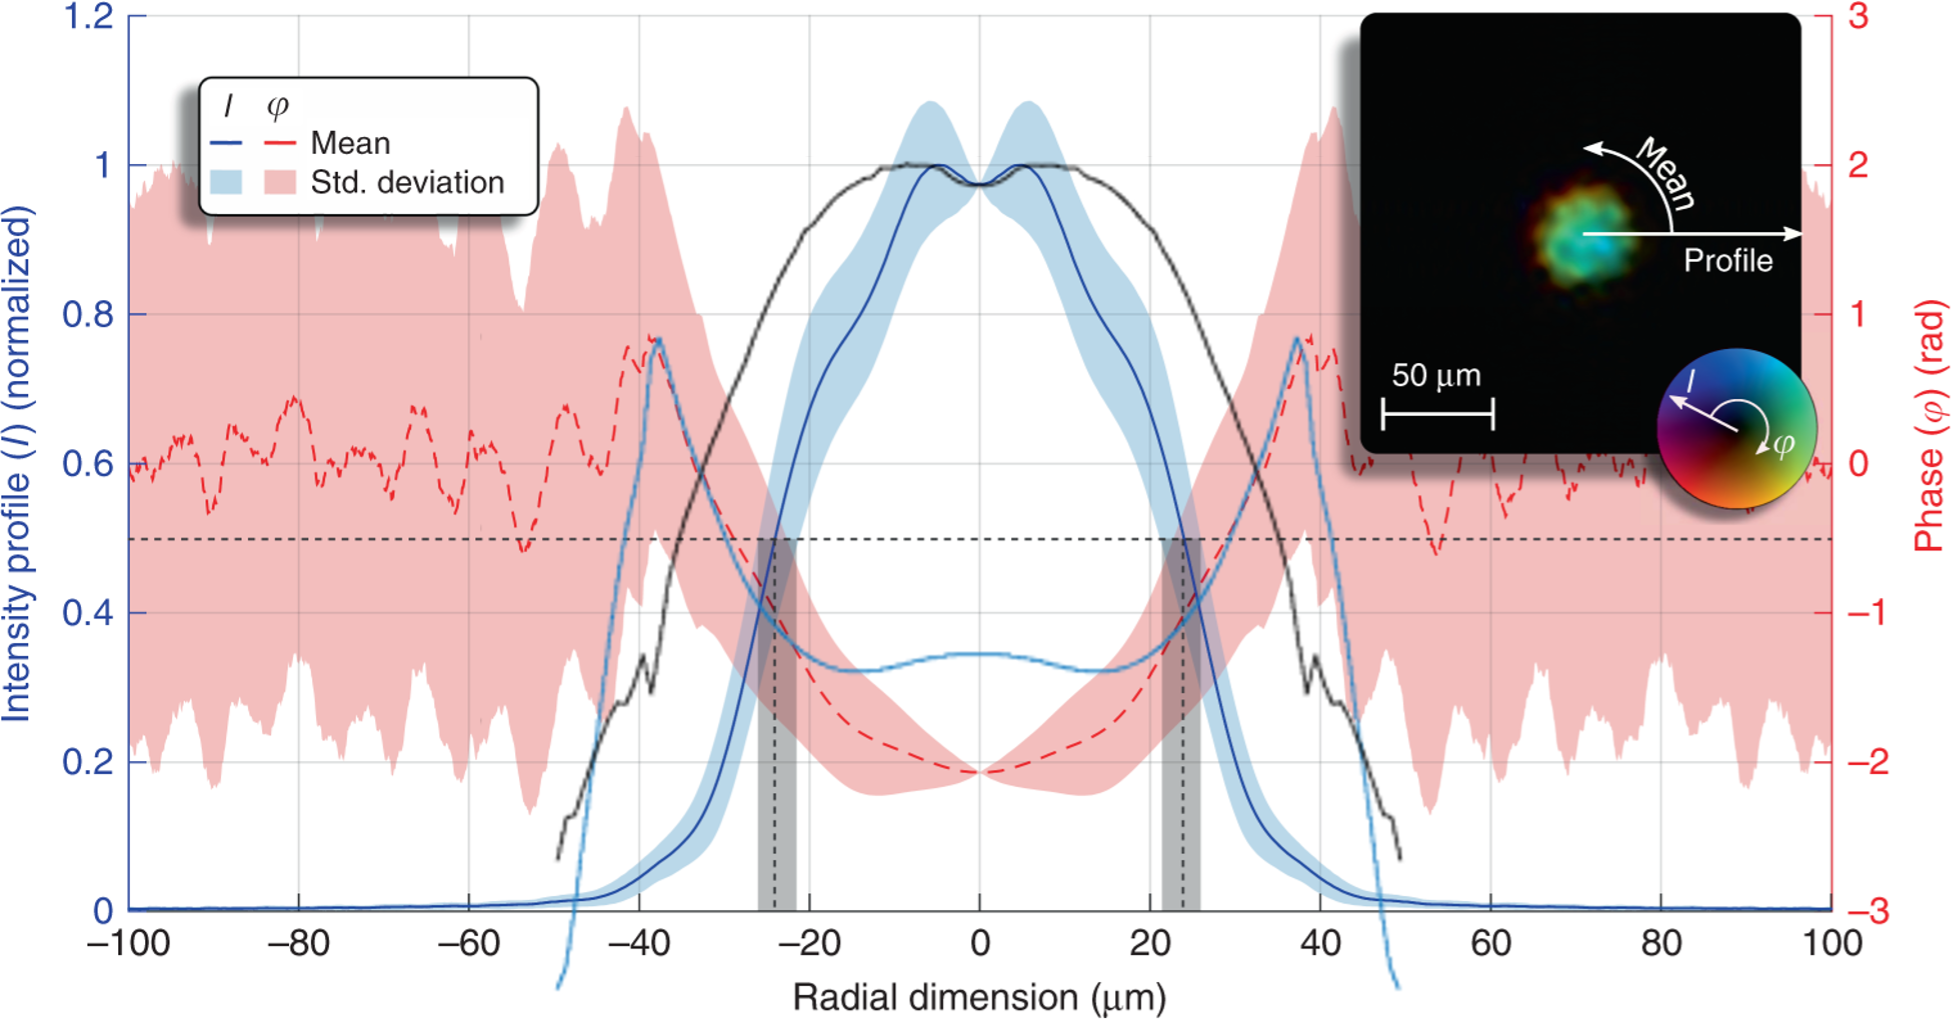
\includegraphics[width=0.7\textwidth]{Figuras/anx_cmp_74.png}
  \caption*{Comparación entre los perfiles radiales de intensidad--fase con $k_{ig}=\qty{5000}{m^{-1}}$, manteniendo los valores de los parámetros $r_{ig,min}=\qty{15}{µm}$, $r_{ig,max}=\qty{25}{µm}$ y $z_{0ig}=\qty{4}{mm}$; y el experimento.}
\end{figure}

\begin{figure}[htbp]
  \centering
  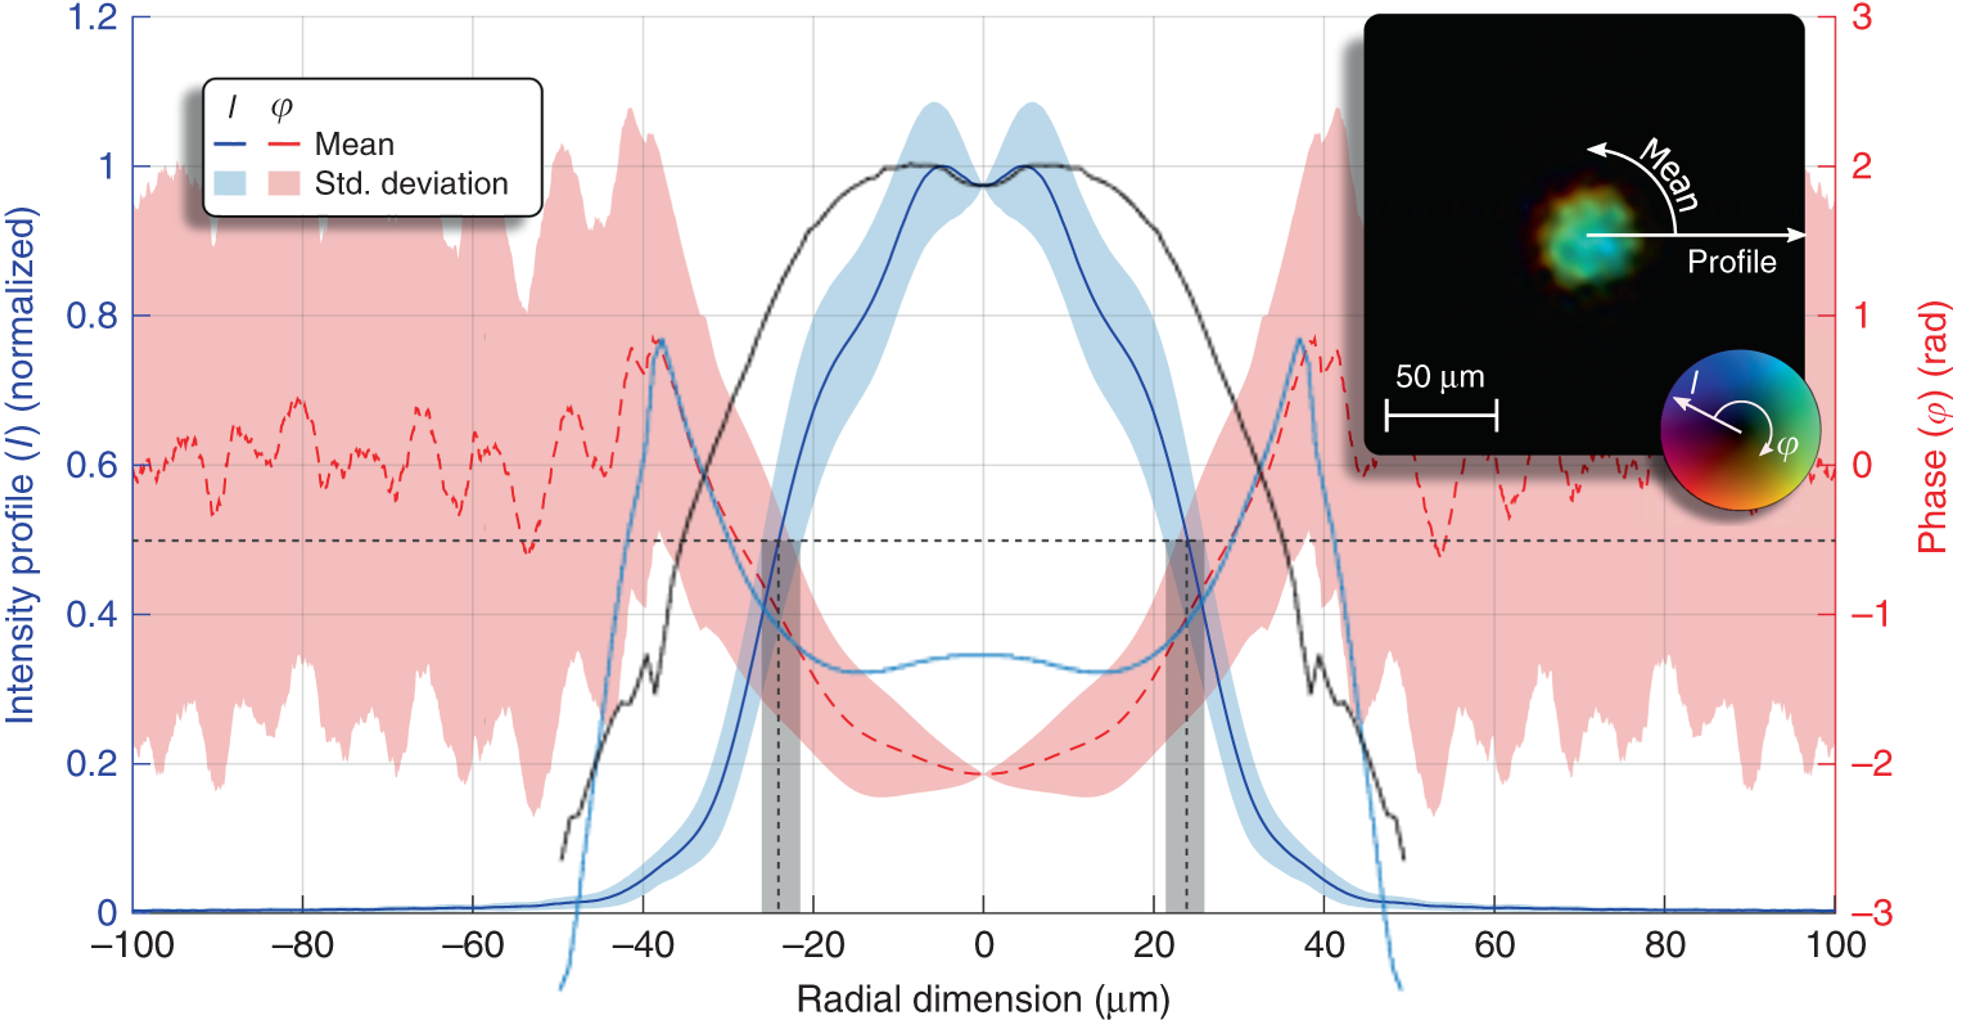
\includegraphics[width=0.75\textwidth]{Figuras/anx_cmp_75.png}
  \caption*{Comparación entre los perfiles radiales de intensidad--fase con $k_{ig}=\qty{6000}{m^{-1}}$, manteniendo los valores de los parámetros $r_{ig,min}=\qty{15}{µm}$, $r_{ig,max}=\qty{25}{µm}$ y $z_{0ig}=\qty{4}{mm}$; y el experimento.}
\end{figure}
